\section{Implementation\label{sec:implementation}}
This chapter describes how the solution concept from Section\ref{subsec:cbr} was realized. It first explains why the \acrshort{cbr} tools presented in Section\ref{sec:exonto} were not used. Then, the overall architecture of the solution to be implemented will be presented. The tools used are then presented. To facilitate understanding of the implementation process, the development strategy is described, followed by the choice of programming languages. For each of these languages, an explanation of their choice is given, followed by a listing of the libraries or packages used. Then the framework's main functions (code snippets) are explained, to give further details on how similarity is calculated. Once the back-end has been explained, a brief presentation of the front-end is given to show how the framework can be used and integrated into applications.

\subsection{Why not myCBR, JCollibri or ProCAKE?\label{sec:whyNot}}
\begin{itemize}
    \item The main reason why these tools will not be used is their age. Apart from ProCAKE, the other tools are quite old and not maintained. Due to their lack of maintenance, these tools are difficult to integrate with modern technologies, so it would be very dangerous to use them for a long-term project. 
    \item The second reason is that these tools are mainly developed in Java. One of our requirements when choosing tools is that they should (if possible) be able to be integrated into Python code.
    \item The third reason is that their documentation is complicated to understand, and there is a lack of articles showing how to use them and integrate them with other tools through APIs, for example. 
    \item Many players are involved in the EP4.0 project. So it's vital to choose solutions that are easy to understand for everyone involved.\\
\end{itemize}
Faced with these problems, it was decided that it would be much simpler to implement a \acrshort{cbr} solution from scratch.


\subsection{Architecture of the Framework \label{subsec:archi-frame}}
Figure\ref{fig:frame-archi} shows the overall structure to be implemented. The chosen architecture is the microservice architecture. Here we have four services:
\begin{itemize}
    \item \textbf{Client}: provides the \acrfull{ui}, which will be used directly by the user
    \item \textbf{Server}: exposes the Reasoning Framework. It exposes an API, which can be consumed to access the functions defined in it. It also features:
        \begin{itemize}
            \item a \textbf{reasoner}: for executing case-based reasoning
            \item a \textbf{storage layer}: to interact with the various storage services
        \end{itemize}
    
    \item two \textbf{storage services}: 
        \begin{itemize}
            \item for \textbf{non-graphical data}
            \item for \textbf{graphical / ontological data}
        \end{itemize}
\end{itemize}


\begin{figure}[h]
\centering
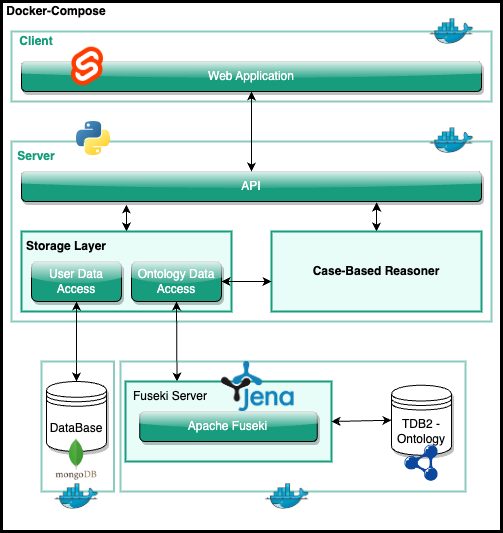
\includegraphics[scale=0.6]{images/SemanticAssistant-Detailled Architecture.drawio.png}
\caption{\label{fig:frame-archi}  Framework architecture}
\end{figure}


\subsection{Used Tools}
    \subsubsection{Protégé \label{subsubsec:protege}}
    Protégé is an ontology development and knowledge management tool that plays a central role in our feasibility study on the use of semantic technologies to support configuration processes in systems engineering. In particular, Protégé facilitates the creation, modification and visualization of ontologies and enables us to define and organize the key attributes relevant for simulations in the automotive industry.
    
    \subsubsection{Apache Jana}
    Apache Jena is a semantic web framework that proves to be very helpful in implementing semantic technologies in our platform. As part of our solution, Apache Jena supports processing RDF data, performing semantic reasoning and executing SPARQL queries to improve the identification of similarities between new and existing simulations in our knowledge graph.
    
    \subsubsection{Apache Fuseki}
    Apache Fuseki is an important component for managing and exposing RDF data as linked data resources. In our study, Apache Fuseki is used to provide an endpoint for querying and retrieving information from the knowledge graph and to ensure seamless integration with other tools and components of our platform.

    
    \subsubsection{\acrshort{tdb2}}
    \acrshort{tdb2}, the native triple store for Apache Jena, is used for persistent storage of RDF data. This ensures efficient data retrieval and management and contributes to the robustness and scalability of our simulation configuration solution.
    
    
    \subsubsection{MongoDB}
    MongoDB is used as a NoSQL database to store additional non-semantic data related to simulations. It complements the semantic aspects by providing a flexible and scalable storage solution for various parameters and attributes related to simulations in the automotive industry.
    
    \subsubsection{Docker}
    Docker is essential for containerizing our platform by creating an isolated and uniform environment for component deployment and execution. This simplifies deployment, scalability, and repeatability across many computer settings.
    
    \subsubsection{Docker Compose}
    Docker Compose is a tool for managing several Docker containers. It allows for the orchestration of various services inside our platform, ensuring that the many components involved in automotive simulation configuration procedures communicate and interact seamlessly. This improves the overall efficiency and reliability of our solution.

    
\subsection{Development Strategy}
Development begins with the creation of the ontology. Once the ontology had been created, all the architecture elements presented in Section\ref{subsec:archi-frame} were parameterized. These are the Front-end, the Back-end, MongoDB and Apache Fuseki. DockerFiles for setting up the containers were then created. Then a Docker-Compose file was defined for orchestration and communication between containers.\\

Once the setup had been done, a set of functions (CRUD) for manipulating the databases were defined in the back-end. The \acrshort{cbr} principles presented in Section\ref{subsec:cbr} were then implemented. This enabled us to:
\begin{itemize}
    \item retrieve cases from the TDB2 database
    \item generate questions for users based on the elements present in the ontology
    \item calculate the similarity between two cases
    \item find the set of cases similar to a problem
\end{itemize}

Once these functions had been fully defined, an API was defined so that they could be accessed and used by other applications.

After completing the back-end implementation, a prototype user interface was coded and integrated with the API.


\subsection{Development of the Ontology \label{subsec:ontologyDev}}
Two options were considered for ontology development. The first was OntoUML, and the second was Protégé. In this section, we will analyze the strengths and weaknesses of each of these tools, and explain why Protégé was chosen.

    \subsubsection{Usage of OntoUML}
    OntoUML (Ontology Unified Modelling Language) is a language designed primarily for the creation of ontologies. It is based on the Unified Modeling Language (UML), with which software developers and modelers are already familiar. OntoUML relies on the Unified Fundamental Ontology (UFO) as its philosophical basis, enabling complex connections and structures to be defined in a precise and semantically rich way, thus ensuring the consistency and clarity of the final ontology.
    
    \paragraph{Advantages}
        \begin{itemize}
            \item \textbf{Intuitive}: OntoUML builds on the established foundation of UML, providing a familiar, user-friendly experience for those familiar with UML diagrams.
            \item \textbf{Formalism}: Based on UFO, OntoUML offers a rigorous, formal framework for knowledge representation, enabling precise, unambiguous descriptions of ideas and their connections.
            \item \textbf{Integration}: Thanks to its UML base, OntoUML interfaces effortlessly with existing software development tools, making it easy to integrate ontology into software applications.
        \end{itemize}
        
    \paragraph{Inconveniences}
        \begin{itemize}
            \item \textbf{Limited tool support}: Although OntoUML is a language, there is no specialized, widely-used ontology editor.
            \item \textbf{Learning Curve}: Mastering OntoUML may require a steep learning curve, especially for those inexperienced with ontological notions and object-oriented modeling.
            \item \textbf{Complexity}: in some cases, the richness of OntoUML can add a complexity that exceeds the needs of the modeling mission.
        \end{itemize}
    
    \subsubsection{Usage of Protégé}
    Protégé is an open-source ontology authoring tool that makes it easy to create, modify and manage ontologies. It supports a variety of ontology languages, including OWL.
    
    \paragraph{Advantages}
    \begin{itemize}
        \item \textbf{User-friendly interface}: Protégé's simple interface makes ontology building easy for ontology experts and professionals alike.
        \item \textbf{Feature-rich}: Protégé's toolbox enables users to create sophisticated and powerful ontologies.
        \item \textbf{Extensibility}: The platform supports the incorporation of plugins, extending its capabilities to meet a wide range of modeling requirements.
        \item \textbf{Community support}: Protégé benefits from a thriving community that provides resources, documentation, and collaboration opportunities.
        \item \textbf{Interoperability}: Protégé supports a variety of ontology languages, enabling the exchange of information with other systems using different forms.
        \item \textbf{Integration}:  Integration with reasoning tools that can detect errors and extract more information from the ontology.
    \end{itemize}
    
    \paragraph{Inconveniences}
    \begin{itemize}
        \item \textbf{Performance limitations}: Large ontologies can cause performance problems in Protégé, reducing application speed and responsiveness.
        \item \textbf{Limited visualizations}: Although Protégé has visualization capabilities, there may be limitations in developing dynamic and interactive visual representations. The representation it provides may be less natural for people used to UML-based techniques such as OntoUML.
    \end{itemize}
    

    \subsubsection{Why Protégé was chosen over OntoUML}
    Protégé was chosen because of its user-friendly interface and widespread use in the ontology development community. The flexibility of the platform and the support of the community were considered essential for the efficient creation and maintenance of the ontology for our feasibility research. In addition, Protégé's interoperability with OWL is consistent with conventional ontology representation standards. The fact that Protégé supports different ontology languages increases the potential for future integration of the ontology developed with other systems.
    
    The graph in Figure\ref{fig:viz-ontology} shows a representation of the ontology developed. It shows the different classes and the relationships between them.
    
    \begin{figure}[p]
         %%%%%%%%%%%%%%%%%%%%%%%%%%%%%%%%%%%%%%%%%%%%%%%%%%%%%%%%%%%%%%%%%%%%
 %        Generated with the experimental alpha version of the TeX exporter of WebVOWL (version 1.1.3) %%% 
 %%%%%%%%%%%%%%%%%%%%%%%%%%%%%%%%%%%%%%%%%%%%%%%%%%%%%%%%%%%%%%%%%%%%

 %   The content can be used as import in other TeX documents. 
 %   Parent document has to use the following packages   
 %   \usepackage{tikz}  
 %   \usepackage{helvet}  
 %   \usetikzlibrary{decorations.markings,decorations.shapes,decorations,arrows,automata,backgrounds,petri,shapes.geometric}  
 %   \usepackage{xcolor}  

 %%%%%%%%%%%%%%% Example Parent Document %%%%%%%%%%%%%%%%%%%%%%%
 %\documentclass{article} 
 %\usepackage{tikz} 
 %\usepackage{helvet} 
 %\usetikzlibrary{decorations.markings,decorations.shapes,decorations,arrows,automata,backgrounds,petri,shapes.geometric} 
 %\usepackage{xcolor} 

 %\begin{document} 
 %\section{Example} 
 %  This is an example. 
 %  \begin{figure} 
 %    \input{<THIS_FILE_NAME>} % << tex file name for the graph 
 %    \caption{A generated graph with TKIZ using alpha version of the TeX exporter of WebVOWL (version 1.1.3) } 
 %  \end{figure} 
 %\end{document} 
 %%%%%%%%%%%%%%%%%%%%%%%%%%%%%%%%%%%%%%%%%%%%%%%%%%%%%%%%%%%%%%%%%%%%

\definecolor{imageBGCOLOR}{HTML}{FFFFFF} 
\definecolor{owlClassColor}{HTML}{AACCFF}
\definecolor{owlObjectPropertyColor}{HTML}{AACCFF}
\definecolor{owlExternalClassColor}{HTML}{AACCFF}
\definecolor{owlDatatypePropertyColor}{HTML}{99CC66}
\definecolor{owlDatatypeColor}{HTML}{FFCC33}
\definecolor{owlThingColor}{HTML}{FFFFFF}
\definecolor{valuesFrom}{HTML}{6699CC}
\definecolor{rdfPropertyColor}{HTML}{CC99CC}
\definecolor{unionColor}{HTML}{6699cc}
\begin{center} 
\resizebox{\linewidth}{!}{
\begin{tikzpicture}[framed]
\clip (-403.03979294983236pt , 597.2174071205975pt ) rectangle (1418.7574536521824pt , -1453.9836880298267pt);
\tikzstyle{dashed}=[dash pattern=on 4pt off 4pt] 
\tikzstyle{dotted}=[dash pattern=on 2pt off 2pt] 
\fontfamily{sans-serif}{\fontsize{12}{12}\selectfont}
 
\tikzset{triangleBlack/.style = {fill=black, draw=black, line width=1pt,scale=0.7,regular polygon, regular polygon sides=3} }
\tikzset{triangleWhite/.style = {fill=white, draw=black, line width=1pt,scale=0.7,regular polygon, regular polygon sides=3} }
\tikzset{triangleBlue/.style  = {fill=valuesFrom, draw=valuesFrom, line width=1pt,scale=0.7,regular polygon, regular polygon sides=3} }
\tikzset{Diamond/.style = {fill=white, draw=black, line width=2pt,scale=1.2,regular polygon, regular polygon sides=4} }
\tikzset{Literal/.style={rectangle,align=center,
font={\fontsize{12pt}{12}\selectfont \sffamily },
black, draw=black, dashed, line width=1pt, fill=owlDatatypeColor, minimum width=80pt,
minimum height = 20pt}}

\tikzset{Datatype/.style={rectangle,align=center,
font={\fontsize{12pt}{12}\selectfont \sffamily },
black, draw=black, line width=1pt, fill=owlDatatypeColor, minimum width=80pt,
minimum height = 20pt}}

\tikzset{owlClass/.style={circle, inner sep=0mm,align=center, 
font={\fontsize{12pt}{12}\selectfont \sffamily },
black, draw=black, line width=1pt, fill=owlClassColor, minimum size=101pt}}

\tikzset{anonymousClass/.style={circle, inner sep=0mm,align=center, 
font={\fontsize{12pt}{12}\selectfont \sffamily },
black, dashed, draw=black, line width=1pt, fill=owlClassColor, minimum size=101pt}}

\tikzset{owlThing/.style={circle, inner sep=0mm,align=center,
font={\fontsize{12pt}{12}\selectfont \sffamily },
black, dashed, draw=black, line width=1pt, fill=owlThingColor, minimum size=62pt}}

\tikzset{owlObjectProperty/.style={rectangle,align=center,
inner sep=0mm,
font={\fontsize{12pt}{12}\selectfont \sffamily },
fill=owlObjectPropertyColor, minimum width=80pt,
minimum height = 25pt}}

\tikzset{rdfProperty/.style={rectangle,align=center,
inner sep=0mm,
font={\fontsize{12pt}{12}\selectfont \sffamily },
fill=rdfPropertyColor, minimum width=80pt,
minimum height = 25pt}}

\tikzset{owlDatatypeProperty/.style={rectangle,align=center,
fill=owlDatatypePropertyColor, minimum width=80pt,
inner sep=0mm,
font={\fontsize{12pt}{12}\selectfont \sffamily },
minimum height = 25pt}}

\tikzset{rdfsSubClassOf/.style={rectangle,align=center,
font={\fontsize{12pt}{12}\selectfont \sffamily },
inner sep=0mm,
fill=imageBGCOLOR, minimum width=80pt,
minimum height = 25pt}}

\tikzset{unionOf/.style={circle, inner sep=0mm,align=center,
font={\fontsize{12pt}{12}\selectfont \sffamily },
black, draw=black, line width=1pt, fill=unionColor, minimum size=25pt}}

\tikzset{disjointWith/.style={circle, inner sep=0mm,align=center,
font={\fontsize{12pt}{12}\selectfont \sffamily },
black, draw=black, line width=1pt, fill=unionColor, minimum size=20pt}}

\tikzset{owlEquivalentClass/.style={circle,align=center,
font={\fontsize{12pt}{12}\selectfont \sffamily },
inner sep=0mm,
black, solid, draw=black, line width=3pt, fill=owlExternalClassColor, minimum size=101pt,
postaction = {draw,line width=1pt, white}}}

\draw [black,line width=2pt, tension=3] plot [smooth] coordinates {(902.2987798847872pt, -180.34888011433011pt) (1000.664063041456pt, -110.31022075523141pt)  (939.1039456624013pt, -214.19233992686026pt)};
\node[triangleBlack, rotate=-226.4379324986707] at (944.0481567382812pt, -209.4827423095703pt)   (marker0) {};
 \node[triangleBlack, rotate=-218.70705033280888] at (906.0565795898438pt, -175.67141723632812pt)   (INV_marker0) {};
 \draw [black,line width=2pt] plot [smooth] coordinates {(560.3248202971527pt, -1203.777924964349pt) (581.9677186799197pt, -1318.389459376423pt)  (603.6106170626867pt, -1433.000993788497pt)};
\node[triangleBlack, rotate=-169.30698282782595] at (602.4463500976562pt, -1426.835693359375pt)   (single_marker1) {};
 \draw [black,line width=2pt] plot [smooth] coordinates {(585.9851344451697pt, -1190.6409425352972pt) (667.1630111163604pt, -1276.1027880179372pt)  (748.3408877875511pt, -1361.564633500577pt)};
\node[triangleBlack, rotate=-136.47209669895497] at (743.6976928710938pt, -1356.6763916015625pt)   (single_marker2) {};
 \draw [black,line width=2pt] plot [smooth] coordinates {(508.4545633661711pt, -1181.9949016677756pt) (419.71540189017804pt, -1241.2800333433704pt)  (330.976240414185pt, -1300.5651650189652pt)};
\node[triangleBlack, rotate=-236.25392002821187] at (336.3327941894531pt, -1296.986572265625pt)   (single_marker3) {};
 \draw [black,line width=2pt] plot [smooth] coordinates {(620.3046061311322pt, -649.5618793084539pt) (589.0629192507387pt, -876.3513147576313pt)  (557.8212323703451pt, -1103.1407502068087pt)};
\node[triangleBlack, rotate=-187.84375689790573] at (558.7576904296875pt, -1096.342529296875pt)   (single_marker4) {};
 \draw [black, dotted ,line width=2pt] plot [smooth] coordinates {(305.38777806162534pt, -871.6634228694224pt) (233.82223549730918pt, -969.3465534548138pt)  (162.25669293299305pt, -1067.0296840402052pt)};
\node[triangleWhite, rotate=-216.22782275612047] at (165.9130859375pt, -1062.0389404296875pt)   (single_marker5) {};
 \draw [black, dotted ,line width=2pt] plot [smooth] coordinates {(500.1597276121157pt, -1148.1552751110546pt) (341.48868237574266pt, -1130.9168823628713pt)  (182.8176371393696pt, -1113.678489614688pt)};
\node[triangleWhite, rotate=83.799849188741] at (188.99072265625pt, -1114.34912109375pt)   (single_marker6) {};
 \draw [black,line width=2pt] plot [smooth] coordinates {(-153.8302594365342pt, -139.77271675135975pt) (-213.9485047026726pt, -61.69899390412324pt)  (-274.066749968811pt, 16.37472894311327pt)};
\node[triangleBlack, rotate=37.59680366535423] at (-270.35992431640625pt, 11.560806274414062pt)   (single_marker7) {};
 \draw [black,line width=2pt] plot [smooth] coordinates {(285.5717160323048pt, -131.52966991783822pt) (206.79558357342324pt, -21.888729561763967pt)  (128.01945111454168pt, 87.75221079431029pt)};
\node[triangleBlack, rotate=35.697035445832725] at (131.5282745361328pt, 82.86862182617188pt)   (single_marker8) {};
 \draw [black,line width=2pt] plot [smooth] coordinates {(678.260462386362pt, -598.4010265410386pt) (838.7622667535156pt, -596.3930818997546pt)  (984.8147799365408pt, -645.8871940882634pt)};
\node[triangleBlack, rotate=-111.14421723936321] at (979.1914672851562pt, -643.7123413085938pt)   (marker9) {};
 \draw [black,line width=2pt, tension=3] plot [smooth] coordinates {(1212.9020245840793pt, 410.1071476754451pt) (1211.4792880104899pt, 278.2967269111869pt)  (1183.061781147008pt, 407.01524346988793pt)};
\node[triangleBlack, rotate=3.82864276258114] at (1183.528076171875pt, 400.09796142578125pt)   (marker10) {};
 \draw [black,line width=2pt, tension=3] plot [smooth] coordinates {(1166.4666080219256pt, 426.1337039448398pt) (1044.1765687597226pt, 472.07962292206105pt)  (1173.723477730408pt, 455.24277198272296pt)};
\node[triangleBlack, rotate=-106.11556471356982] at (1167.37939453125pt, 457.0715026855469pt)   (marker11) {};
 \draw [black, dotted ,line width=2pt] plot [smooth] coordinates {(577.8006155637627pt, -586.6160939267745pt) (440.77272080033265pt, -552.2013407872923pt)  (303.7448260369026pt, -517.78658764781pt)};
\node[triangleWhite, rotate=75.9022646991013] at (310.11395263671875pt, -519.3861694335938pt)   (single_marker12) {};
 \draw [black, dotted ,line width=2pt] plot [smooth] coordinates {(306.1178878754975pt, -223.1086093220136pt) (284.8055476616099pt, -339.1555961096436pt)  (263.49320744772234pt, -455.2025828972737pt)};
\node[triangleWhite, rotate=-190.40665839867168] at (264.7532043457031pt, -448.34173583984375pt)   (single_marker13) {};
 \draw [black, dotted ,line width=2pt] plot [smooth] coordinates {(214.90159341408997pt, -795.8335014978484pt) (180.0420310076604pt, -927.3529539146026pt)  (145.18246860123082pt, -1058.8724063313568pt)};
\node[triangleWhite, rotate=-194.84499899205565] at (146.7509002685547pt, -1052.9549560546875pt)   (single_marker14) {};
 \draw [black,line width=2pt] plot [smooth] coordinates {(345.4561850634702pt, -214.09869595658193pt) (471.2972797983816pt, -385.99326325122706pt)  (597.1383745332931pt, -557.8878305458721pt)};
\node[triangleBlack, rotate=-143.79245786536686] at (593.5532836914062pt, -552.99072265625pt)   (single_marker15) {};
 \draw [black,line width=2pt] plot [smooth] coordinates {(389.2289868836813pt, 304.63132290407543pt) (396.0014459890827pt, 402.11077538873553pt)  (402.7739050944841pt, 499.5902278733956pt)};
\node[triangleBlack, rotate=-3.9740888488974946] at (402.32830810546875pt, 493.1768493652344pt)   (single_marker16) {};
 \draw [black, dotted ,line width=2pt] plot [smooth] coordinates {(870.896683935559pt, -182.44429095161146pt) (814.1293278209178pt, -53.09489080902701pt)  (757.3619717062763pt, 76.25450933355745pt)};
\node[triangleWhite, rotate=23.69516309466522] at (759.9805297851562pt, 70.28800201416016pt)   (single_marker17) {};
 \draw [black, dotted ,line width=2pt] plot [smooth] coordinates {(433.4867664531697pt, 235.9529879035693pt) (561.2804162667824pt, 188.35450076478594pt)  (689.0740660803951pt, 140.75601362600258pt)};
\node[triangleWhite, rotate=-110.4285476355988] at (682.757568359375pt, 143.10867309570312pt)   (single_marker18) {};
 \draw [black,line width=2pt, tension=3] plot [smooth] coordinates {(1207.2369831513463pt, 461.9283120390655pt) (1320.7140569227793pt, 527.4117934024047pt)  (1225.1077052232258pt, 437.83189544593614pt)};
\node[triangleBlack, rotate=-235.5581162907556] at (1230.342529296875pt, 441.42742919921875pt)   (marker19) {};
 \node[triangleBlack, rotate=-231.30715014571666] at (1211.9229736328125pt, 465.6753845214844pt)   (INV_marker19) {};
 \draw [black,line width=2pt] plot [smooth] coordinates {(1077.6767323707447pt, -687.0629572432058pt) (1165.1640583061499pt, -735.7684981918105pt)  (1252.6513842415548pt, -784.4740391404154pt)};
\node[triangleBlack, rotate=-119.10487337407828] at (1247.1796875pt, -781.4279174804688pt)   (single_marker20) {};
 \draw [black,line width=2pt] plot [smooth] coordinates {(529.7632844860893pt, -1200.094970165666pt) (481.58144731288877pt, -1306.1304692221024pt)  (433.3996101396882pt, -1412.165968278539pt)};
\node[triangleBlack, rotate=-204.43646616227278] at (436.2697448730469pt, -1405.849609375pt)   (single_marker21) {};
 \draw [black,line width=2pt, tension=3] plot [smooth] coordinates {(1173.1221179271831pt, 454.60146744655015pt) (1147.8670177449767pt, 583.217435263306pt)  (1201.7050390644454pt, 463.7128130804862pt)};
\node[triangleBlack, rotate=-164.4344491745153] at (1199.967041015625pt, 469.9364013671875pt)   (marker22) {};
 \draw [black,line width=2pt, tension=3] plot [smooth] coordinates {(337.2016030709791pt, 265.9385369209909pt) (270.3350153407938pt, 365.56246465872647pt)  (372.0000725808532pt, 301.84210944198605pt)};
\node[triangleBlack, rotate=-138.00115553902506] at (367.7633361816406pt, 306.53729248046875pt)   (marker23) {};
 \node[triangleBlack, rotate=-130.18722723504808] at (332.6228332519531pt, 269.81597900390625pt)   (INV_marker23) {};
 \draw [black,line width=2pt] plot [smooth] coordinates {(377.3962825184002pt, 203.43355281041747pt) (350.5121751876869pt, 40.403222999770406pt)  (323.62806785697364pt, -122.62710681087665pt)};
\node[triangleBlack, rotate=-189.3639043481923] at (324.6798400878906pt, -116.24906921386719pt)   (single_marker24) {};
 \node[triangleBlack, rotate=-9.363904348192307] at (376.4200439453125pt, 197.51348876953125pt)   (INV_single_marker24) {};
 \draw [black,line width=2pt] plot [smooth] coordinates {(1083.4178058572377pt, -653.8416678900917pt) (1177.9439334832985pt, -638.0300093853582pt)  (1272.4700611093592pt, -622.2183508806247pt)};
\node[triangleBlack, rotate=-80.50404541472629] at (1265.8828125pt, -623.3201904296875pt)   (single_marker25) {};
 \draw [black,line width=2pt] plot [smooth] coordinates {(599.1827011078692pt, -1169.9746750209715pt) (696.7988027786198pt, -1202.9253807813357pt)  (794.4149044493703pt, -1235.8760865417pt)};
\node[triangleBlack, rotate=-108.65225162239754] at (788.6780395507812pt, -1233.9395751953125pt)   (single_marker26) {};
 \draw [black,line width=2pt] plot [smooth] coordinates {(942.2375107112941pt, -225.17734634365956pt) (1033.5005468295394pt, -218.05608760699798pt)  (1124.763582947785pt, -210.9348288703364pt)};
\node[triangleBlack, rotate=-85.53796174463935] at (1118.7010498046875pt, -211.4078826904297pt)   (single_marker27) {};
 \draw [black,line width=2pt] plot [smooth] coordinates {(-173.69395221202586pt, -181.6464018483957pt) (-263.3670831510683pt, -184.22382442667413pt)  (-353.04021409011074pt, -186.8012470049526pt)};
\node[triangleBlack, rotate=-268.35353532678124] at (-346.6225280761719pt, -186.61679077148438pt)   (single_marker28) {};
 \draw [black,line width=2pt] plot [smooth] coordinates {(1221.9041820430425pt, 418.4837165028311pt) (1299.2974422889695pt, 372.16437453583734pt)  (1376.6907025348964pt, 325.8450325688436pt)};
\node[triangleBlack, rotate=-120.9001089914728] at (1371.2071533203125pt, 329.1269226074219pt)   (single_marker29) {};
 \draw [black,line width=2pt] plot [smooth] coordinates {(264.3370589145335pt, -173.78958844202853pt) (96.30755063181883pt, -176.5643311215124pt)  (-71.72195765089583pt, -179.33907380099626pt)};
\node[triangleBlack, rotate=-269.0537854349364] at (-65.61792755126953pt, -179.23828125pt)   (single_marker30) {};
 \draw [black,line width=2pt] plot [smooth] coordinates {(-156.7885107151389pt, -218.12842598673575pt) (-224.65778771353007pt, -293.71368176854276pt)  (-292.52706471192124pt, -369.2989375503497pt)};
\node[triangleBlack, rotate=-221.9214493833223] at (-288.40576171875pt, -364.7091064453125pt)   (single_marker31) {};
 \draw [black,line width=2pt] plot [smooth] coordinates {(656.9014692091589pt, -557.5342218616042pt) (759.3282598805449pt, -414.09191325169115pt)  (861.7550505519308pt, -270.64960464177807pt)};
\node[triangleBlack, rotate=-35.52908995237802] at (857.9683227539062pt, -275.9527282714844pt)   (single_marker32) {};
 \node[triangleBlack, rotate=-215.5288359291804] at (660.38818359375pt, -552.6513061523438pt)   (INV_single_marker32) {};
 \draw [black,line width=2pt] plot [smooth] coordinates {(587.3132168629131pt, -630.7391457226494pt) (481.3964723723052pt, -714.7809858495739pt)  (375.4797278816973pt, -798.8228259764983pt)};
\node[triangleBlack, rotate=-231.56848124675193] at (380.5068359375pt, -794.833984375pt)   (single_marker33) {};
 \draw [black,line width=2pt] plot [smooth] coordinates {(676.24573582011pt, -613.2458347081035pt) (829.7667772661633pt, -657.7740037232004pt)  (982.1290509909377pt, -661.1319550852667pt)};
\node[triangleBlack, rotate=-89.36527140529863] at (975.7022094726562pt, -661.2031860351562pt)   (marker34) {};
 \draw [black,line width=2pt] plot [smooth] coordinates {(600.8983901681595pt, -1143.799638096911pt) (693.7649888381455pt, -1125.4924951482458pt)  (786.6315875081316pt, -1107.1853521995808pt)};
\node[triangleBlack, rotate=-78.84918205268572] at (780.44287109375pt, -1108.4052734375pt)   (single_marker35) {};
 \draw [black,line width=2pt] plot [smooth] coordinates {(579.4240345687923pt, -616.7108604165147pt) (427.6162678826564pt, -672.7873863093625pt)  (275.80850119652047pt, -728.8639122022104pt)};
\node[triangleBlack, rotate=-249.72678242428245] at (282.0629577636719pt, -726.5535278320312pt)   (single_marker36) {};
 \definecolor{Node37_COLOR}{HTML}{3366cc} 
 \node[owlClass ,minimum size=100pt , fill=Node37_COLOR  , text=white] at (736.86658881785pt, 122.95503695645263pt)   (Node37) {Package\\ {\small (external) }};
\definecolor{Node38_COLOR}{HTML}{3366cc} 
 \node[owlClass ,minimum size=100pt , fill=Node38_COLOR  , text=white] at (385.6942437157149pt, 253.75396457311925pt)   (Node38) {LoadCaseTem...\\ {\small (external) }};
\definecolor{Node39_COLOR}{HTML}{3366cc} 
 \node[owlClass ,minimum size=100pt , fill=Node39_COLOR  , text=white] at (550.861385564373pt, -1153.6636215863869pt)   (Node39) {PhysicalBasicS...\\ {\small (external) }};
\definecolor{Node40_COLOR}{HTML}{3366cc} 
 \node[owlClass ,minimum size=100pt , fill=Node40_COLOR  , text=white] at (254.2809886635609pt, -505.3636736457089pt)   (Node40) {Model\\ {\small (external) }};
\definecolor{Node41_COLOR}{HTML}{3366cc} 
 \node[owlClass ,minimum size=100pt , fill=Node41_COLOR  , text=white] at (227.96808282820842pt, -746.5357646898494pt)   (Node41) {MathematicalB...\\ {\small (external) }};
\definecolor{Node42_COLOR}{HTML}{3366cc} 
 \node[owlClass ,minimum size=100pt , fill=Node42_COLOR  , text=white] at (1033.1166694152685pt, -662.2556843297236pt)   (Node42) {Task\\ {\small (external) }};
\node[Literal ,minimum width=53pt  , text=black] at (814.1127052454607pt, -1101.7678957834778pt)   (Node43) {Literal};
\node[Literal ,minimum width=53pt  , text=black] at (315.1765356684126pt, -1311.1206803146788pt)   (Node44) {Literal};
\node[Literal ,minimum width=53pt  , text=black] at (605.6845446116141pt, -1443.983627188065pt)   (Node45) {Literal};
\definecolor{Node46_COLOR}{HTML}{3366cc} 
 \node[owlClass ,minimum size=100pt , fill=Node46_COLOR  , text=white] at (98.2610604871875pt, 129.1700594500505pt)   (Node46) {Numeric\\ {\small (external) }};
\node[Literal ,minimum width=53pt  , text=black] at (758.5283160684359pt, -1372.2896790093791pt)   (Node47) {Literal};
\definecolor{Node48_COLOR}{HTML}{3366cc} 
 \node[owlClass ,minimum size=100pt , fill=Node48_COLOR  , text=white] at (132.11597918711234pt, -1108.1701431393558pt)   (Node48) {BasicStructure\\ {\small (external) }};
\node[Literal ,minimum width=53pt  , text=black] at (821.862381224733pt, -1245.141092166898pt)   (Node49) {Literal};
\definecolor{Node50_COLOR}{HTML}{3366cc} 
 \node[owlClass ,minimum size=100pt , fill=Node50_COLOR  , text=white] at (335.52849180750604pt, -830.522963770272pt)   (Node50) {LogicalBasicSt...\\ {\small (external) }};
\node[Datatype ,minimum width=49pt  , text=black] at (1271.48761055687pt, -794.960456256366pt)   (Node51) {string};
\node[Datatype ,minimum width=49pt  , text=black] at (-302.1743414531089pt, -380.0430019095122pt)   (Node52) {string};
\node[Datatype ,minimum width=49pt  , text=black] at (403.53797139017087pt, 510.58782313478685pt)   (Node53) {string};
\node[Datatype ,minimum width=49pt  , text=black] at (1297.956357902339pt, -617.9551843724711pt)   (Node54) {string};
\node[Datatype ,minimum width=49pt  , text=black] at (-378.53980128258144pt, -187.5341667890441pt)   (Node55) {string};
\node[Datatype ,minimum width=49pt  , text=black] at (1150.2605524357714pt, -208.94529921575133pt)   (Node56) {string};
\node[owlThing ,minimum size=60pt  , text=black] at (1195.3042352774632pt, 434.4036044442819pt)   (Node57) {Thing};
\node[Literal ,minimum width=53pt  , text=black] at (428.4419872951228pt, -1423.0763868781328pt)   (Node58) {Literal};
\node[Datatype ,minimum width=49pt  , text=black] at (1394.2573922182257pt, 315.33148779653874pt)   (Node59) {string};
\node[Datatype ,minimum width=49pt  , text=black] at (-282.377042383764pt, 27.167051039546344pt)   (Node60) {string};
\definecolor{Node61_COLOR}{HTML}{3366cc} 
 \node[owlClass ,minimum size=100pt , fill=Node61_COLOR  , text=white] at (627.2644529371044pt, -599.0390079288757pt)   (Node61) {CoreModel\\ {\small (external) }};
\definecolor{Node62_COLOR}{HTML}{3366cc} 
 \node[owlClass ,minimum size=100pt , fill=Node62_COLOR  , text=white] at (315.33010665965895pt, -172.94751857357844pt)   (Node62) {BasicModel\\ {\small (external) }};
\definecolor{Node63_COLOR}{HTML}{3366cc} 
 \node[owlClass ,minimum size=100pt , fill=Node63_COLOR  , text=white] at (-122.71500539602128pt, -180.18114366944636pt)   (Node63) {Solver\\ {\small (external) }};
\definecolor{Node64_COLOR}{HTML}{3366cc} 
 \node[owlClass ,minimum size=100pt , fill=Node64_COLOR  , text=white] at (891.3920668239854pt, -229.14481857450664pt)   (Node64) {LoadCase\\ {\small (external) }};
\definecolor{property0_COLOR}{HTML}{3366cc} 
 \definecolor{inv_property0_COLOR}{HTML}{3366cc} 
 % Createing Inverse Property 
\node[owlObjectProperty ,minimum width=80pt , fill=inv_property0_COLOR  , text=white] at (1000.664063041456pt, -124.31022075523141pt)   (property0) {hasLCChild\\ {\small (inverse functional) }};
% owlObjectProperty vs owlObjectProperty
% ,minimum width=80pt vs ,minimum width=90pt
% , fill=inv_property0_COLOR  vs , fill=property0_COLOR 
% , text=white vs , text=white
\node[owlObjectProperty ,minimum width=90pt , fill=property0_COLOR  , text=white] at (1000.664063041456pt, -96.31022075523141pt)   (property0) {hasLCParent\\ {\small (functional) }};
\definecolor{property1_COLOR}{HTML}{3366cc} 
 \node[owlDatatypeProperty ,minimum width=73pt , fill=property1_COLOR  , text=white] at (581.9677186799197pt, -1318.389459376423pt)   (property1) {behaviour};
\definecolor{property2_COLOR}{HTML}{3366cc} 
 \node[owlDatatypeProperty ,minimum width=110pt , fill=property2_COLOR  , text=white] at (667.1630111163604pt, -1276.1027880179372pt)   (property2) {timeDependency};
\definecolor{property3_COLOR}{HTML}{3366cc} 
 \node[owlDatatypeProperty ,minimum width=102pt , fill=property3_COLOR  , text=white] at (419.715401890178pt, -1241.2800333433704pt)   (property3) {thermodynamic};
\definecolor{property4_COLOR}{HTML}{3366cc} 
 \node[owlObjectProperty ,minimum width=120pt , fill=property4_COLOR  , text=white] at (589.0629192507387pt, -876.3513147576313pt)   (property4) {hasPhysicalBasicS...};
\node[rdfsSubClassOf ,minimum width=82pt  , text=black] at (233.82223549730918pt, -969.3465534548138pt)   (property5) {Subclass of};
\node[rdfsSubClassOf ,minimum width=82pt  , text=black] at (341.48868237574266pt, -1130.9168823628713pt)   (property6) {Subclass of};
\definecolor{property7_COLOR}{HTML}{3366cc} 
 \node[owlDatatypeProperty ,minimum width=65pt , fill=property7_COLOR  , text=white] at (-213.9485047026726pt, -61.69899390412324pt)   (property7) {software};
\definecolor{property8_COLOR}{HTML}{3366cc} 
 \node[owlObjectProperty ,minimum width=84pt , fill=property8_COLOR  , text=white] at (206.79558357342324pt, -21.888729561763967pt)   (property8) {hasNumeric};
\definecolor{property9_COLOR}{HTML}{3366cc} 
 \node[owlObjectProperty ,minimum width=105pt , fill=property9_COLOR  , text=white] at (838.7622667535156pt, -596.3930818997546pt)   (property9) {hasOutOfScope};
\definecolor{property10_COLOR}{HTML}{3366cc} 
 \node[owlObjectProperty ,minimum width=98pt , fill=property10_COLOR  , text=white] at (1211.4792880104899pt, 278.2967269111869pt)   (property10) {hasCoreModel\\ {\small (functional) }};
\definecolor{property11_COLOR}{HTML}{3366cc} 
 \node[owlObjectProperty ,minimum width=101pt , fill=property11_COLOR  , text=white] at (1044.1765687597226pt, 472.07962292206105pt)   (property11) {hasBasicModel\\ {\small (functional) }};
\node[rdfsSubClassOf ,minimum width=82pt  , text=black] at (440.77272080033265pt, -552.2013407872923pt)   (property12) {Subclass of};
\node[rdfsSubClassOf ,minimum width=82pt  , text=black] at (284.8055476616099pt, -339.1555961096436pt)   (property13) {Subclass of};
\node[rdfsSubClassOf ,minimum width=82pt  , text=black] at (180.04203100766037pt, -927.3529539146026pt)   (property14) {Subclass of};
\definecolor{property15_COLOR}{HTML}{3366cc} 
 \node[owlObjectProperty ,minimum width=117pt , fill=property15_COLOR  , text=white] at (471.2972797983816pt, -385.99326325122706pt)   (property15) {bmHasCoreModel\\ {\small (functional) }};
\definecolor{property16_COLOR}{HTML}{3366cc} 
 \node[owlDatatypeProperty ,minimum width=72pt , fill=property16_COLOR  , text=white] at (396.00144598908264pt, 402.1107753887355pt)   (property16) {lctVersion\\ {\small (functional) }};
\node[rdfsSubClassOf ,minimum width=82pt  , text=black] at (814.1293278209178pt, -53.09489080902701pt)   (property17) {Subclass of};
\node[rdfsSubClassOf ,minimum width=82pt  , text=black] at (561.2804162667825pt, 188.35450076478594pt)   (property18) {Subclass of};
\definecolor{property19_COLOR}{HTML}{3366cc} 
 \definecolor{inv_property19_COLOR}{HTML}{3366cc} 
 % Createing Inverse Property 
\node[owlObjectProperty ,minimum width=80pt , fill=inv_property19_COLOR  , text=white] at (1320.7140569227793pt, 513.4117934024047pt)   (property19) {hasChild\\ {\small (inverse functional) }};
% owlObjectProperty vs owlObjectProperty
% ,minimum width=80pt vs ,minimum width=75pt
% , fill=inv_property19_COLOR  vs , fill=property19_COLOR 
% , text=white vs , text=white
\node[owlObjectProperty ,minimum width=75pt , fill=property19_COLOR  , text=white] at (1320.7140569227793pt, 541.4117934024047pt)   (property19) {hasParent\\ {\small (functional) }};
\definecolor{property20_COLOR}{HTML}{3366cc} 
 \node[owlDatatypeProperty ,minimum width=78pt , fill=property20_COLOR  , text=white] at (1165.1640583061499pt, -735.7684981918105pt)   (property20) {description};
\definecolor{property21_COLOR}{HTML}{3366cc} 
 \node[owlDatatypeProperty ,minimum width=90pt , fill=property21_COLOR  , text=white] at (481.5814473128887pt, -1306.1304692221024pt)   (property21) {physicNature};
\definecolor{property22_COLOR}{HTML}{3366cc} 
 \node[owlObjectProperty ,minimum width=120pt , fill=property22_COLOR  , text=white] at (1147.8670177449767pt, 583.217435263306pt)   (property22) {caemHasBasicModel\\ {\small (functional) }};
\definecolor{property23_COLOR}{HTML}{3366cc} 
 \definecolor{inv_property23_COLOR}{HTML}{3366cc} 
 % Createing Inverse Property 
\node[owlObjectProperty ,minimum width=80pt , fill=inv_property23_COLOR  , text=white] at (270.3350153407938pt, 351.56246465872647pt)   (property23) {hasLCTChild\\ {\small (inverse functional) }};
% owlObjectProperty vs owlObjectProperty
% ,minimum width=80pt vs ,minimum width=97pt
% , fill=inv_property23_COLOR  vs , fill=property23_COLOR 
% , text=white vs , text=white
\node[owlObjectProperty ,minimum width=97pt , fill=property23_COLOR  , text=white] at (270.3350153407938pt, 379.56246465872647pt)   (property23) {hasLCTParent\\ {\small (functional) }};
\definecolor{property24_COLOR}{HTML}{3366cc} 
 \definecolor{inv_property24_COLOR}{HTML}{3366cc} 
 % Createing Inverse Property 
\node[owlObjectProperty ,minimum width=80pt , fill=inv_property24_COLOR  , text=white] at (350.5121751876869pt, 26.403222999770406pt)   (property24) {hasLoadC...\\ {\small (functional, inv...) }};
% owlObjectProperty vs owlObjectProperty
% ,minimum width=80pt vs ,minimum width=120pt
% , fill=inv_property24_COLOR  vs , fill=property24_COLOR 
% , text=white vs , text=white
\node[owlObjectProperty ,minimum width=120pt , fill=property24_COLOR  , text=white] at (350.5121751876869pt, 54.403222999770406pt)   (property24) {lctHasBasicModel\\ {\small (functional, inverse funct...) }};
\definecolor{property25_COLOR}{HTML}{3366cc} 
 \node[owlDatatypeProperty ,minimum width=50pt , fill=property25_COLOR  , text=white] at (1177.9439334832985pt, -638.0300093853582pt)   (property25) {name};
\definecolor{property26_COLOR}{HTML}{3366cc} 
 \node[owlDatatypeProperty ,minimum width=77pt , fill=property26_COLOR  , text=white] at (696.7988027786198pt, -1202.9253807813357pt)   (property26) {complexity};
\definecolor{property27_COLOR}{HTML}{3366cc} 
 \node[owlDatatypeProperty ,minimum width=69pt , fill=property27_COLOR  , text=white] at (1033.5005468295394pt, -218.05608760699798pt)   (property27) {lcVersion\\ {\small (functional) }};
\definecolor{property28_COLOR}{HTML}{3366cc} 
 \node[owlDatatypeProperty ,minimum width=46pt , fill=property28_COLOR  , text=white] at (-263.3670831510683pt, -184.22382442667413pt)   (property28) {input};
\definecolor{property29_COLOR}{HTML}{3366cc} 
 \node[owlDatatypeProperty ,minimum width=62pt , fill=property29_COLOR  , text=white] at (1299.2974422889693pt, 372.16437453583734pt)   (property29) {version\\ {\small (functional) }};
\definecolor{property30_COLOR}{HTML}{3366cc} 
 \node[owlObjectProperty ,minimum width=73pt , fill=property30_COLOR  , text=white] at (96.30755063181883pt, -176.5643311215124pt)   (property30) {hasSolver\\ {\small (functional) }};
\definecolor{property31_COLOR}{HTML}{3366cc} 
 \node[owlDatatypeProperty ,minimum width=53pt , fill=property31_COLOR  , text=white] at (-224.6577877135301pt, -293.7136817685427pt)   (property31) {output};
\definecolor{property32_COLOR}{HTML}{3366cc} 
 \definecolor{inv_property32_COLOR}{HTML}{3366cc} 
 % Createing Inverse Property 
\node[owlObjectProperty ,minimum width=80pt , fill=inv_property32_COLOR  , text=white] at (759.3282598805449pt, -428.09191325169115pt)   (property32) {lcHasCor...\\ {\small (functional, inv...) }};
% owlObjectProperty vs owlObjectProperty
% ,minimum width=80pt vs ,minimum width=120pt
% , fill=inv_property32_COLOR  vs , fill=property32_COLOR 
% , text=white vs , text=white
\node[owlObjectProperty ,minimum width=120pt , fill=property32_COLOR  , text=white] at (759.3282598805449pt, -400.09191325169115pt)   (property32) {hasLoadCase\\ {\small (functional, inverse funct...) }};
\definecolor{property33_COLOR}{HTML}{3366cc} 
 \node[owlObjectProperty ,minimum width=120pt , fill=property33_COLOR  , text=white] at (481.3964723723052pt, -714.7809858495739pt)   (property33) {hasLogicalBasicSt...};
\definecolor{property34_COLOR}{HTML}{3366cc} 
 \node[owlObjectProperty ,minimum width=83pt , fill=property34_COLOR  , text=white] at (829.7667772661633pt, -657.7740037232004pt)   (property34) {hasInScope};
\definecolor{property35_COLOR}{HTML}{3366cc} 
 \node[owlDatatypeProperty ,minimum width=80pt , fill=property35_COLOR  , text=white] at (693.7649888381454pt, -1125.4924951482458pt)   (property35) {physicType};
\definecolor{property36_COLOR}{HTML}{3366cc} 
 \node[owlObjectProperty ,minimum width=120pt , fill=property36_COLOR  , text=white] at (427.6162678826564pt, -672.7873863093625pt)   (property36) {hasMathematicalB...};
\end{tikzpicture}
}
 \end{center}

         \caption{\label{fig:viz-ontology}  Visualization of a Systematic Map as a Bubble Plot (each color represent different years of publication)}
    \end{figure}

    
\subsection{Used Programming Languages}
    \subsubsection{Python}
        \paragraph{Advantages}
        \begin{itemize}
            \item \textbf{Versatility}: Python's versatility allows for seamless integration with various libraries and frameworks, making it suitable for a wide range of applications.
            \item \textbf{Rapid Development}: Python's syntax and extensive libraries enable rapid prototyping and development, crucial for an efficient master thesis project timeline.
            \item \textbf{Community Support}: The large and active Python community provides extensive documentation, support, and a wealth of resources for problem-solving.
            \item \textbf{Interdisciplinary Integration}: Python's popularity in scientific computing, data analysis, and artificial intelligence domains aligns with the interdisciplinary nature of your thesis.
        \end{itemize}
        
        \paragraph{Used Libraries / Package}
        \begin{table}[h]
            \centering
    	    {\rowcolors{2}{teal!10}{white}
    	    \begin{tabular}{ | m{2.5cm} | m{12cm} | }
                \hline
                \rowcolor{teal!30} Libraries / Packages & Description \\
                
                \hline
                FastAPI & A modern, fast web framework for building APIs with automatic OpenAPI and JSON Schema generation.\\

                \hline
                Uvicorn & A production-grade ASGI (Asynchronous Server Gateway Interface) server used to run FastAPI applications, ensuring efficient handling of asynchronous requests.\\

                \hline
                Pydantic & A data validation library used for defining the data schema in FastAPI, enhancing API request and response handling.\\

                \hline
                pip, setuptools, wheel & Essential tools for package management, distribution, and installation in Python.\\

                \hline
                sparqlwrapper & Facilitates SPARQL query execution in Python, essential for querying semantic knowledge graphs.\\

                \hline
                rdflib & A library for working with RDF (Resource Description Framework) data, supporting semantic data representation.\\

                \hline
                openpyxl & A library for reading and writing Excel files, facilitating data exchange with other applications.\\

                \hline
                levenshtein & A library for calculating Levenshtein distance, beneficial for string similarity comparisons.\\

                \hline
                rapidfuzz & Offers efficient fuzzy string matching, valuable for handling variations in input data.\\

                \hline
                pymongo & A Python driver for MongoDB, supporting integration with MongoDB databases\\
                
                \hline
            \end{tabular}}
            \caption{\label{tab:python-libs} Used Python libraries}
        \end{table}
    
    \subsubsection{JavaScript / TypeScript}
        \paragraph{Advantages}
        \begin{itemize}
            \item Front-end Development: JavaScript and TypeScript are fundamental for building interactive and dynamic user interfaces, enhancing the user experience.
            \item Asynchronous Operations: Asynchronous capabilities of JavaScript and TypeScript are crucial for responsive and efficient web applications.
            \item Widespread Adoption: JavaScript is universally supported in web browsers.
            \item TypeScript: TypeScript, a superset of JavaScript, adds optional static typing, enhancing code reliability and maintainability for larger projects.
            \item Ecosystem: The vast ecosystem of JavaScript libraries and frameworks provides flexibility and choice in front-end development.
        \end{itemize}
        
        \paragraph{Used Libraries / Package}
        \begin{table}[h]
            \centering
    	    {\rowcolors{2}{teal!10}{white}
    	    \begin{tabular}{ | m{2.5cm} | m{12cm} | }
                \hline
                \rowcolor{teal!30} Libraries / Packages & Description \\
                
                \hline
                Svelte & A modern JavaScript framework for building user interfaces with a focus on simplicity and performance. \\

                \hline
                SvelteKit & A full-stack framework built on Svelte, facilitating the creation of complex, scalable web applications and enabling the development of both server-side rendered (SSR) and statically generated applications. \\

                \hline
                Axios & A popular HTTP client for making asynchronous requests, crucial for communicating with backend APIs. \\

                \hline
                Tailwind & A utility-first CSS framework that streamlines the styling process and promotes consistency in the user interface.\\

                \hline
            \end{tabular}}
            \caption{\label{tab:js-libs} Used JavaScript libraries}
        \end{table}
        
\subsection{Framework's main Functions and Classes}
All the codes presented in this section are simplified versions. Full versions can be found in the Appendix.\\

\subsubsection{Extract the schema of a graph}
 When the backend server is launched, one of the first functions to be executed is to extract the ontology schema. To do this, the graph is traversed from an input class considered to be the root. The \textbf{create\_schema\_from\_class} function shown in Listing\ref{lst:create-schema} (see \textbf{Appendix\ref{annex:create-schema-full}} for a full version) is used recursively. It extracts the attributes (\textbf{Data Properties}) of the class and is then used on each of the classes linked by a relationship to the one being studied (\textbf{Object Properties}).\\

An important point to note is that in an ontology, classes can be subclasses of another (\textbf{rdfs:subClassOf}). When creating the schema for a class, it is therefore important to check whether it has a parent class. If it does, the properties (Data Properties, Object Properties) of its parent should be added to its schema.
The user can also exclude certain classes from the analysis. This is made possible by the \textbf{EXCLUDED\_CLASSES} global variable, which is a list of classes to be ignored.\\

\begin{lstlisting}[language=Python, caption=Function to create the schema of the ontology, label={lst:create-schema}]
def create_schema_from_class(
        self, class_uri: str, depth: int, visited: dict[str, bool]
    ) -> Node:
        visited[class_uri] = True
        node = Node(None, class_uri, depth)

        # Get all DataProperties of the instance
        data_properties = get_class_data_properties(...)
        # Get all DataProperties of the superClass
        super_data_properties = get_super_class_data_properties(...)
        data_properties += super_data_properties

        # Add all data properties to the node
        for property_uri, type_uri, type_list in data_properties:
            property_suffix_uri = ...
            type = ...
            node.addAttribute(...)

        # Get all ObjectProperties of the instance
        object_properties = get_class_object_properties(class_uri)
        # Get all ObjectProperties of his super class
        super_object_properties = get_super_class_object_properties(class_uri)
        object_properties += super_object_properties

        # Add edges
        for property_uri, child_class_name_uri in object_properties:
            child_class_name_turtle_uri = extractSuffixURI(...)
            # Check if the class is not already visited and is not in the list of excluded classes
            if (...):
                property_suffix_uri = ...
                node.addEdge(...)

        return node
\end{lstlisting}


\subsubsection{Generate the list of questions}
Once the ontology schema has been extracted, it is searched (Depth search) using the recursive function \textbf{collectQuestionsFromClass}. For each attribute of a class, the \textbf{generateQuestion} function is used, and a question is generated based on the type of the attribute.

\subsubsection{Get the similar cases}
Listing\ref{lst:comp-sim} shows the main function of our framework. This function takes as its parameters the problem (target: Node), the list of attributes that must work, and the list of answers already given. To do this, for each graph in our ontology, the mandatory attributes are checked. If the graph respects these attributes, the function presented in Listing\ref{lst:comp-sim-node} (see \textbf{Appendix\ref{annex:comp-sim-full}} for a full version) is used to calculate the similarity between the target graph and that of the current iteration.\\


\begin{lstlisting}[language=Python, caption=Function to find the similarity between one case and all the cases in the data-base, label={lst:comp-sim}]
def computeSimilarity(
        self, target: Node, mandatories: list[str], responsesStack: dict[str, Any]
    ) -> list[Similarity]:
        similarities = []

        for graphKey, graph in self.ontology.graphs.items():
            # Check if the graph respect the mandatories
            check = checkValidGraphByMandatories(...)
            if check:
                simi = Similarity(self.computeSimilarityForNode(...), graph)
                similarities.append(simi)

        mean = self.similarityMean(similarities)

        # Get only the most similar
        similarities = list(filter(..., similarities))

        # order by similarity descending
        similarities.sort(key=lambda x: x.value, reverse=True)

        return similarities
\end{lstlisting}
    
    
    
\subsubsection{Get the similar cases} 
Here the principle of local-to-global calculation presented in Section\ref{subsec:similarity} is implemented. First we iterate over the set of Node target attributes and for each pair of values, the function presented in Listing\ref{lst:comp-sim-node} (see \textbf{Appendix\ref{annex:comp-sim-node-full}} for a full version) is called. This calculates the similarity value between two attributes according to their type. Then, for each Edge in our graph, the function is used iteratively.
After iterating over all the attributes and edges (child nodes), the similarity value between the two nodes is calculated by applying the same weight to each attribute and child.\\

\begin{lstlisting}[language=Python, caption=Function to find the similarity between one case and all the cases in the data-base, label={lst:comp-sim-node}]
def computeSimilarityForNode(self, node: Node, target: Node) -> float:
        # Local computation
        attributSimilarity = 0
        numberOfAttribute = 0
        for key, targetAttribute in target.attributes.items():
            if targetAttribute.value is not None:
                nodeAttribute = node.getAttribute(key)

                if nodeAttribute is None:
                    continue

                sim = self.computeSimilarityForAttribute(...)
                attributSimilarity += sim
                numberOfAttribute += 1

        # Global computation
        childSimilarity = 0
        numberOfEdges = 0
        for key, targetEdges in target.edges.items():
            nodeEdges = node.getEdge(key)

            if nodeEdges is None:
                continue

            # iterate over all the edeges of this node with the same URI
            collectorSim = [0]
            for targetEdge in targetEdges:
                for nodeEdge in nodeEdges:
                    if nodeEdge is not None:
                        collectorSim.append(
                            self.computeSimilarityForNode(...)
                        )

            sim = max(collectorSim)
            childSimilarity += sim
            numberOfEdges += 1

        if (numberOfAttribute + numberOfEdges) == 0:
            return 0

        nodeSimilarity = (attributSimilarity + childSimilarity) / (
            numberOfAttribute + numberOfEdges
        )

        return nodeSimilarity
\end{lstlisting}



\subsubsection{Find the similarity value between two attributes} 
Calculating the similarity between two attributes depends largely on their type. In the function presented in Listing\ref{lst:comp-sim-att} (see \textbf{Appendix\ref{annex:comp-sim-att-full}} for a full version), a distinction is made between cases based on the type of attributes. Depending on the type, a specific utility function is used.\\

\begin{lstlisting}[language=Python, caption=Function to compute the similarity value between two attributes, label={lst:comp-sim-att}]
def computeSimilarityForAttribute(
        self, nodeAttribute: DataObject, targetAttribute: DataObject
    ) -> float:
        similarity = 0

        match nodeAttribute.type:
            case "string":
                similarity = computeStringLevensteinSimilarity(
                    nodeAttribute.value, targetAttribute.value
                )
            case "int":
                similarity = computeNumericSigmoidSimilarity(...)
            case "double":
                similarity = computeNumericSigmoidSimilarity(...)
            case "decimal":
                similarity = computeNumericSigmoidSimilarity(...)
            case "float":
                similarity = computeNumericSigmoidSimilarity(...)
            case "boolean":
                similarity = self.computeEqualSimilarity(...)
            case "date":
                similarity = computeStringSortRatio(...)
            case _:
                similarity = self.computeEqualSimilarity(...)

        return similarity
\end{lstlisting}
    

\subsection{Similarity Measures}
For the same type, there are numerous functions for calculating similarity. The choice of one depends on the case and the purpose. In this section, various functions for \textbf{String} and \textbf{Numeric} will be presented, along with the cases in which each of them is appropriate.
    
    \subsubsection{String}
    The function in Listing\ref{lst:leven-string} uses Levenshtein's algorithm to calculate how different two Strings are from each other. It is suitable for long texts or when you want to make a comparison while allowing a certain degree of error.\\
    
\begin{lstlisting}[language=Python, caption=Levenstein distance between two strings, label={lst:leven-string}]
# Compute the Levenstein distance between the two strings
def computeStringLevensteinSimilarity(nodeValue: str, targetValue: str) -> float:
    return fuzz.partial_ratio(nodeValue, targetValue)
\end{lstlisting}
    
    
    The function in Listing\ref{lst:leven-string-ratio} works like the previous function, but ignores special characters such as full stops or commas.\\
    
\begin{lstlisting}[language=Python, caption=Levenstein distance between two strings without considering special characters, label={lst:leven-string-ratio}]
def computeStringSortRatio(nodeValue: str, targetValue: str) -> float:
    return fuzz.token_sort_ratio(nodeValue, targetValue)
\end{lstlisting}





    \subsubsection{Numeric}
    
    \textbf{Exponential similarity} in Listing\ref{lst:expo-sim-num} is useful when you want to emphasize the sensitivity to proximity. It is suitable for cases where small differences between numeric values should result in significantly higher similarity scores.\\
    
\begin{lstlisting}[language=Python, caption=Function to compute the similarity value between two attributes, label={lst:expo-sim-num}]
# Compute the Exponential similarity between two numeric values
def computeNumericExponentialSimilarity(value1, value2):
    num1 = int(value1)
    num2 = int(value2)
    return math.exp(-abs(num1 - num2))
\end{lstlisting}
    
    
    \textbf{Fuzzy similarity} in Listing\ref{lst:fuzzy-sim-num} is beneficial when dealing with uncertain or imprecise numeric data. It can handle situations where the exact values may not be known, and there is a need to capture the degree of similarity despite the fuzziness in the data.\\
\begin{lstlisting}[language=Python, caption=Function to compute the similarity value between two attributes, label={lst:fuzzy-sim-num}]
# Compute the Fuzzy similarity between two numeric values
def computeNumericFuzzySimilarity(value1, value2):
    num1 = int(value1)
    num2 = int(value2)
    return 1 - abs(num1 - num2) / (num1 + num2)
\end{lstlisting}

    
    \textbf{Sigmoid similarity} in Listing\ref{lst:sigmo-sim-num} is appropriate when you expect the similarity to saturate at a certain point, indicating that beyond a specific difference threshold, additional proximity has a diminishing impact.\\

\begin{lstlisting}[language=Python, caption=Function to compute the similarity value between two attributes, label={lst:sigmo-sim-num}]
# Compute the sigmoid similarity between two numeric values
def computeNumericSigmoidSimilarity(value1, value2):
    num1 = int(value1)
    num2 = int(value2)
    return 1 / (1 + math.exp(-(num1 - num2)))
\end{lstlisting}
        
In summary, the choice of similarity computation method depends on the nature of the data and the desired characteristics of the similarity measure. Exponential similarity emphasizes proximity sensitivity, fuzzy similarity accommodates uncertainty, and sigmoid similarity is suitable for situations where similarity saturates with increasing proximity.

\subsection{Web Application}
As already explained in the previous chapters, a prototype \acrshort{ui} has been set up in order to demonstrate the use of the \acrshort{cbr} mechanism in practical cases. In this section, the different views and elements of this \acrshort{ui} will be presented, along with their usefulness.

    \subsubsection{The home page}
    Figure\ref{fig:proto-home} shows the home view of the \acrshort{ui}. Here the user can create a new account in which to work or choose an existing account. Each account has a list of configuration processes.
    
    \begin{figure}[H]
    \centering
    \frame{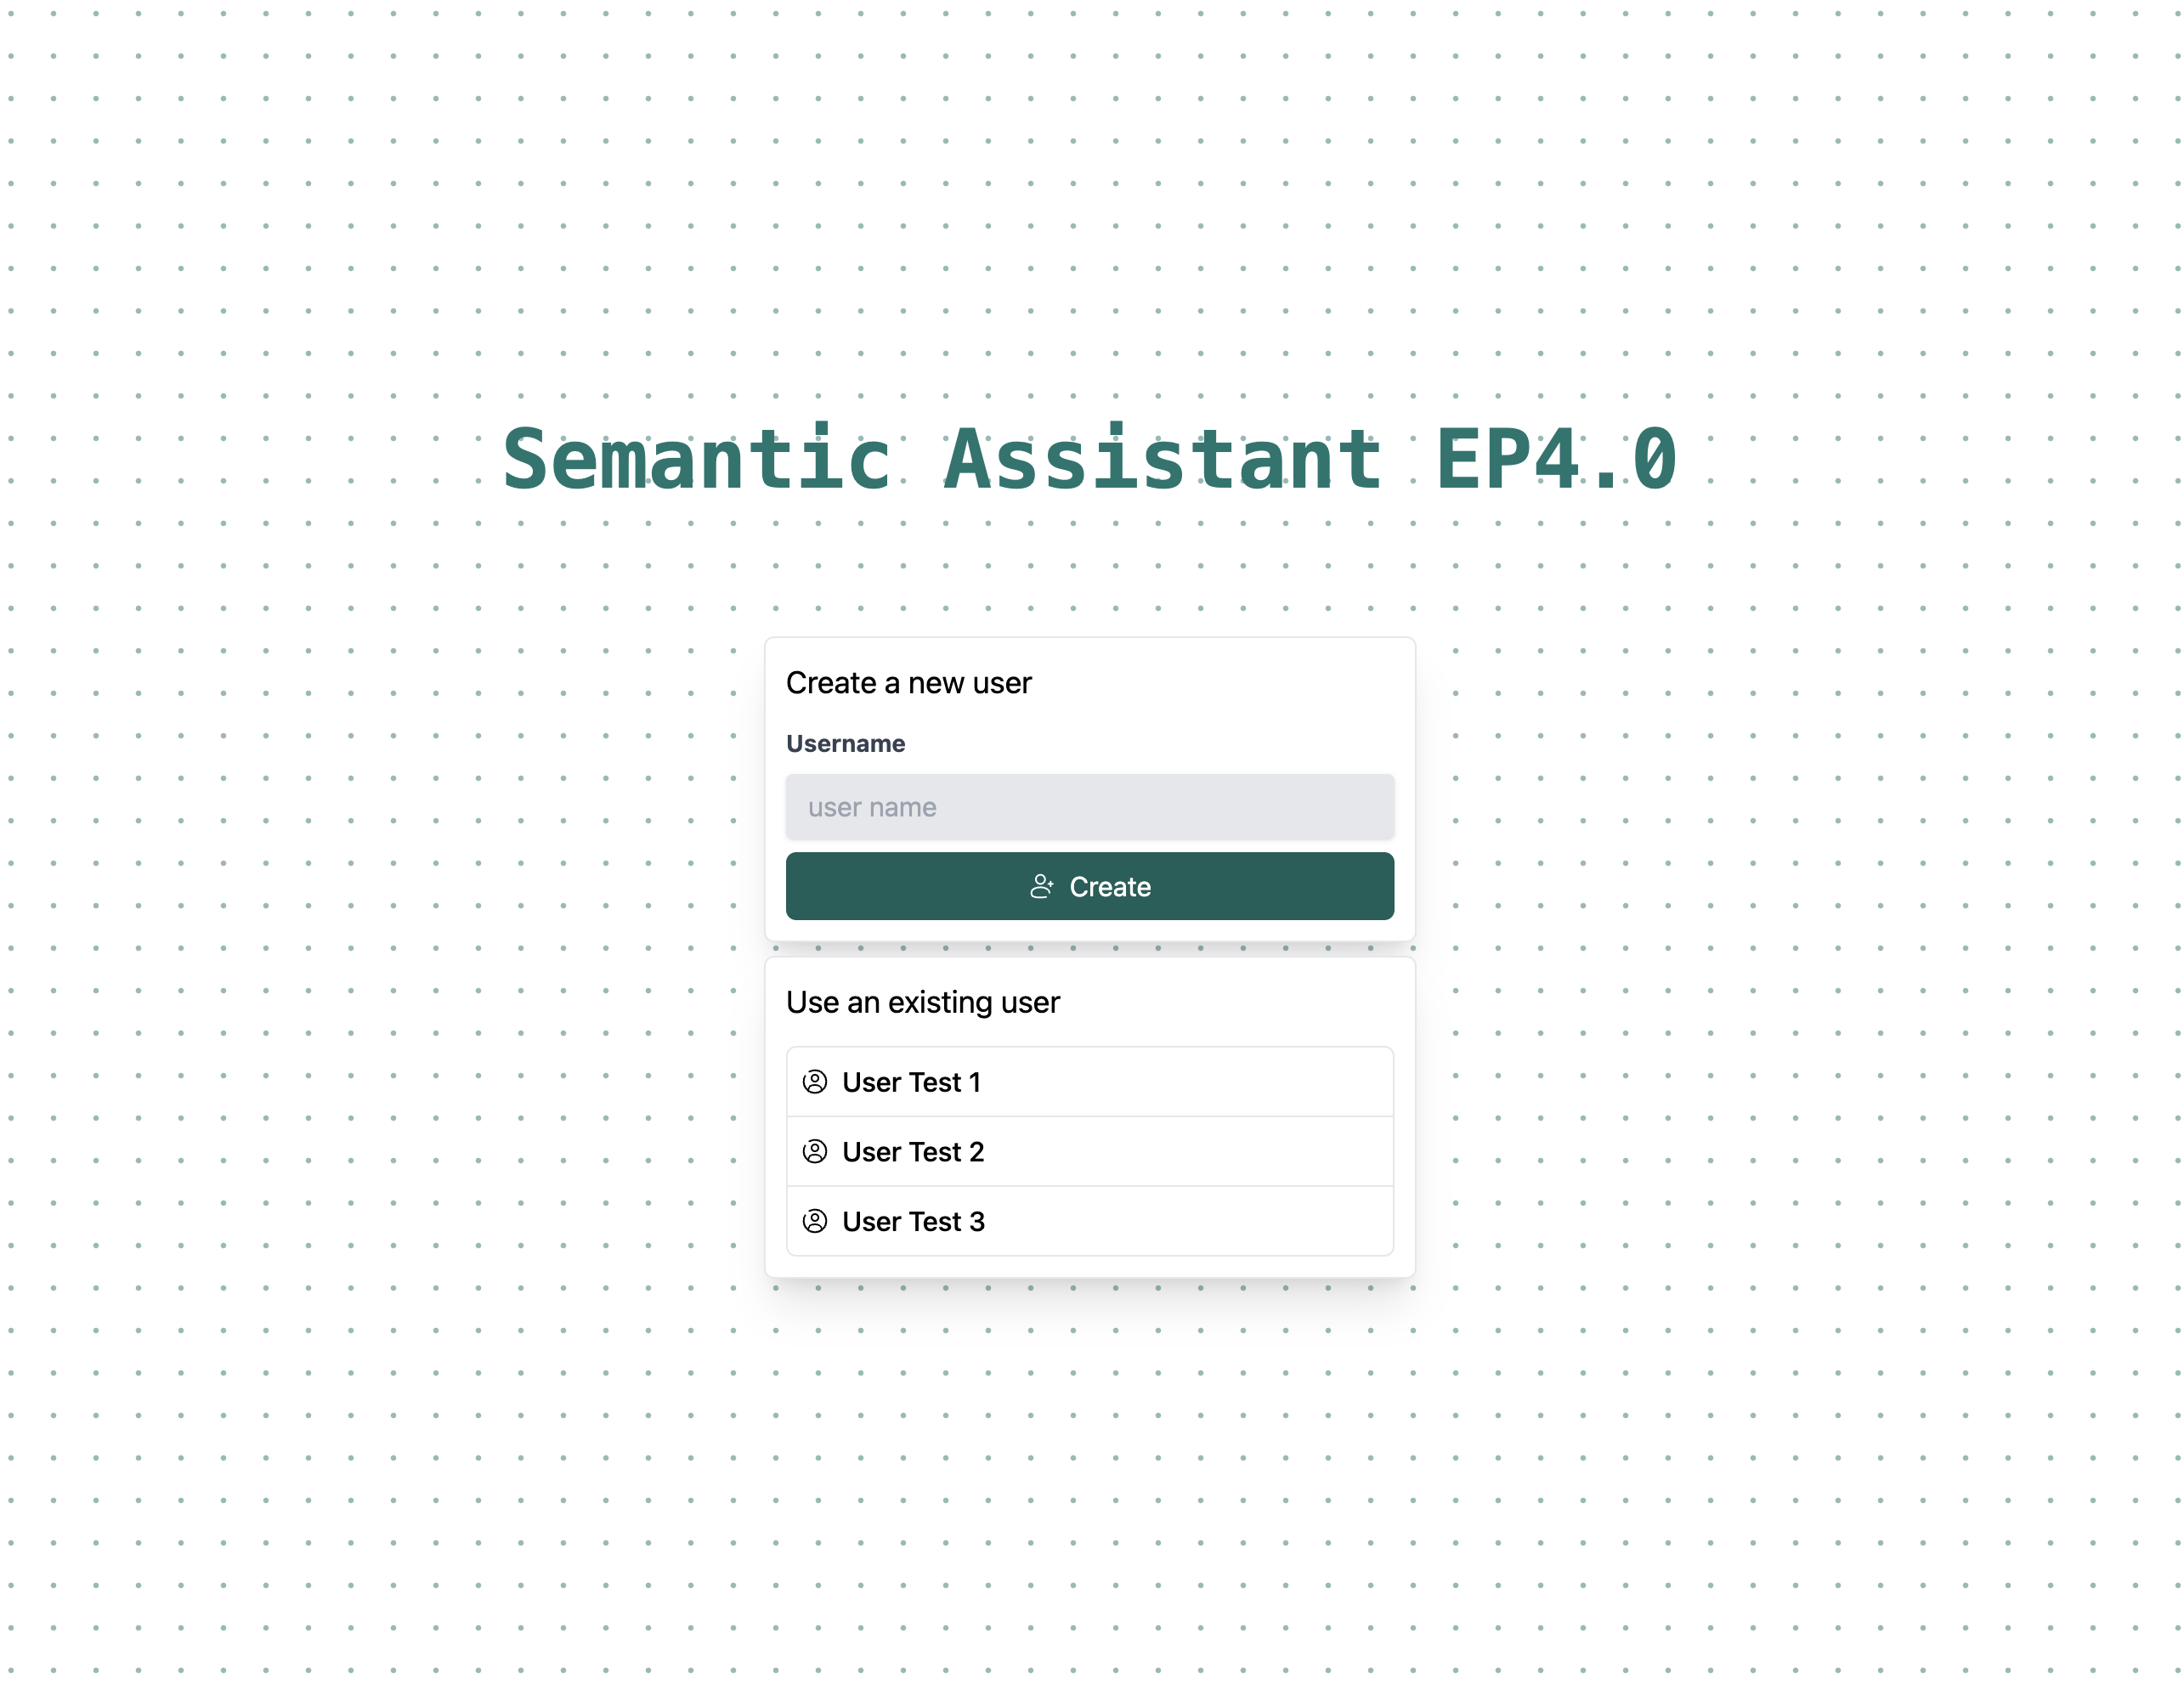
\includegraphics[width=\textwidth]{images/proto-home.png}}
    \caption{\label{fig:proto-home}  Home view of the \acrshort{ui} prototype}
    \end{figure}
    
    
    \subsubsection{The working page}
    Figure\ref{fig:proto-demo} shows the working view. This is where all operations are performed. 
    
    \begin{itemize}
        \item The sidebar \textbf{(1)} lists all the processes associated with the current user. It can also be used to create and delete a process.
        \item The box at the bottom left \textbf{(2)} shows the name of the current user and provides a button for logging out and going to the home page (see Figure\ref{fig:proto-home}).
        \item The title bar \textbf{(3)} shows the name of the selected configuration and allows you to modify or delete it.
        \item The buttons at the bottom right \textbf{(4)} are used to manage the zoom percentage of the decision tree shown in the center of the work area.
    \end{itemize}
    
    \begin{figure}[h]
    \centering
    \frame{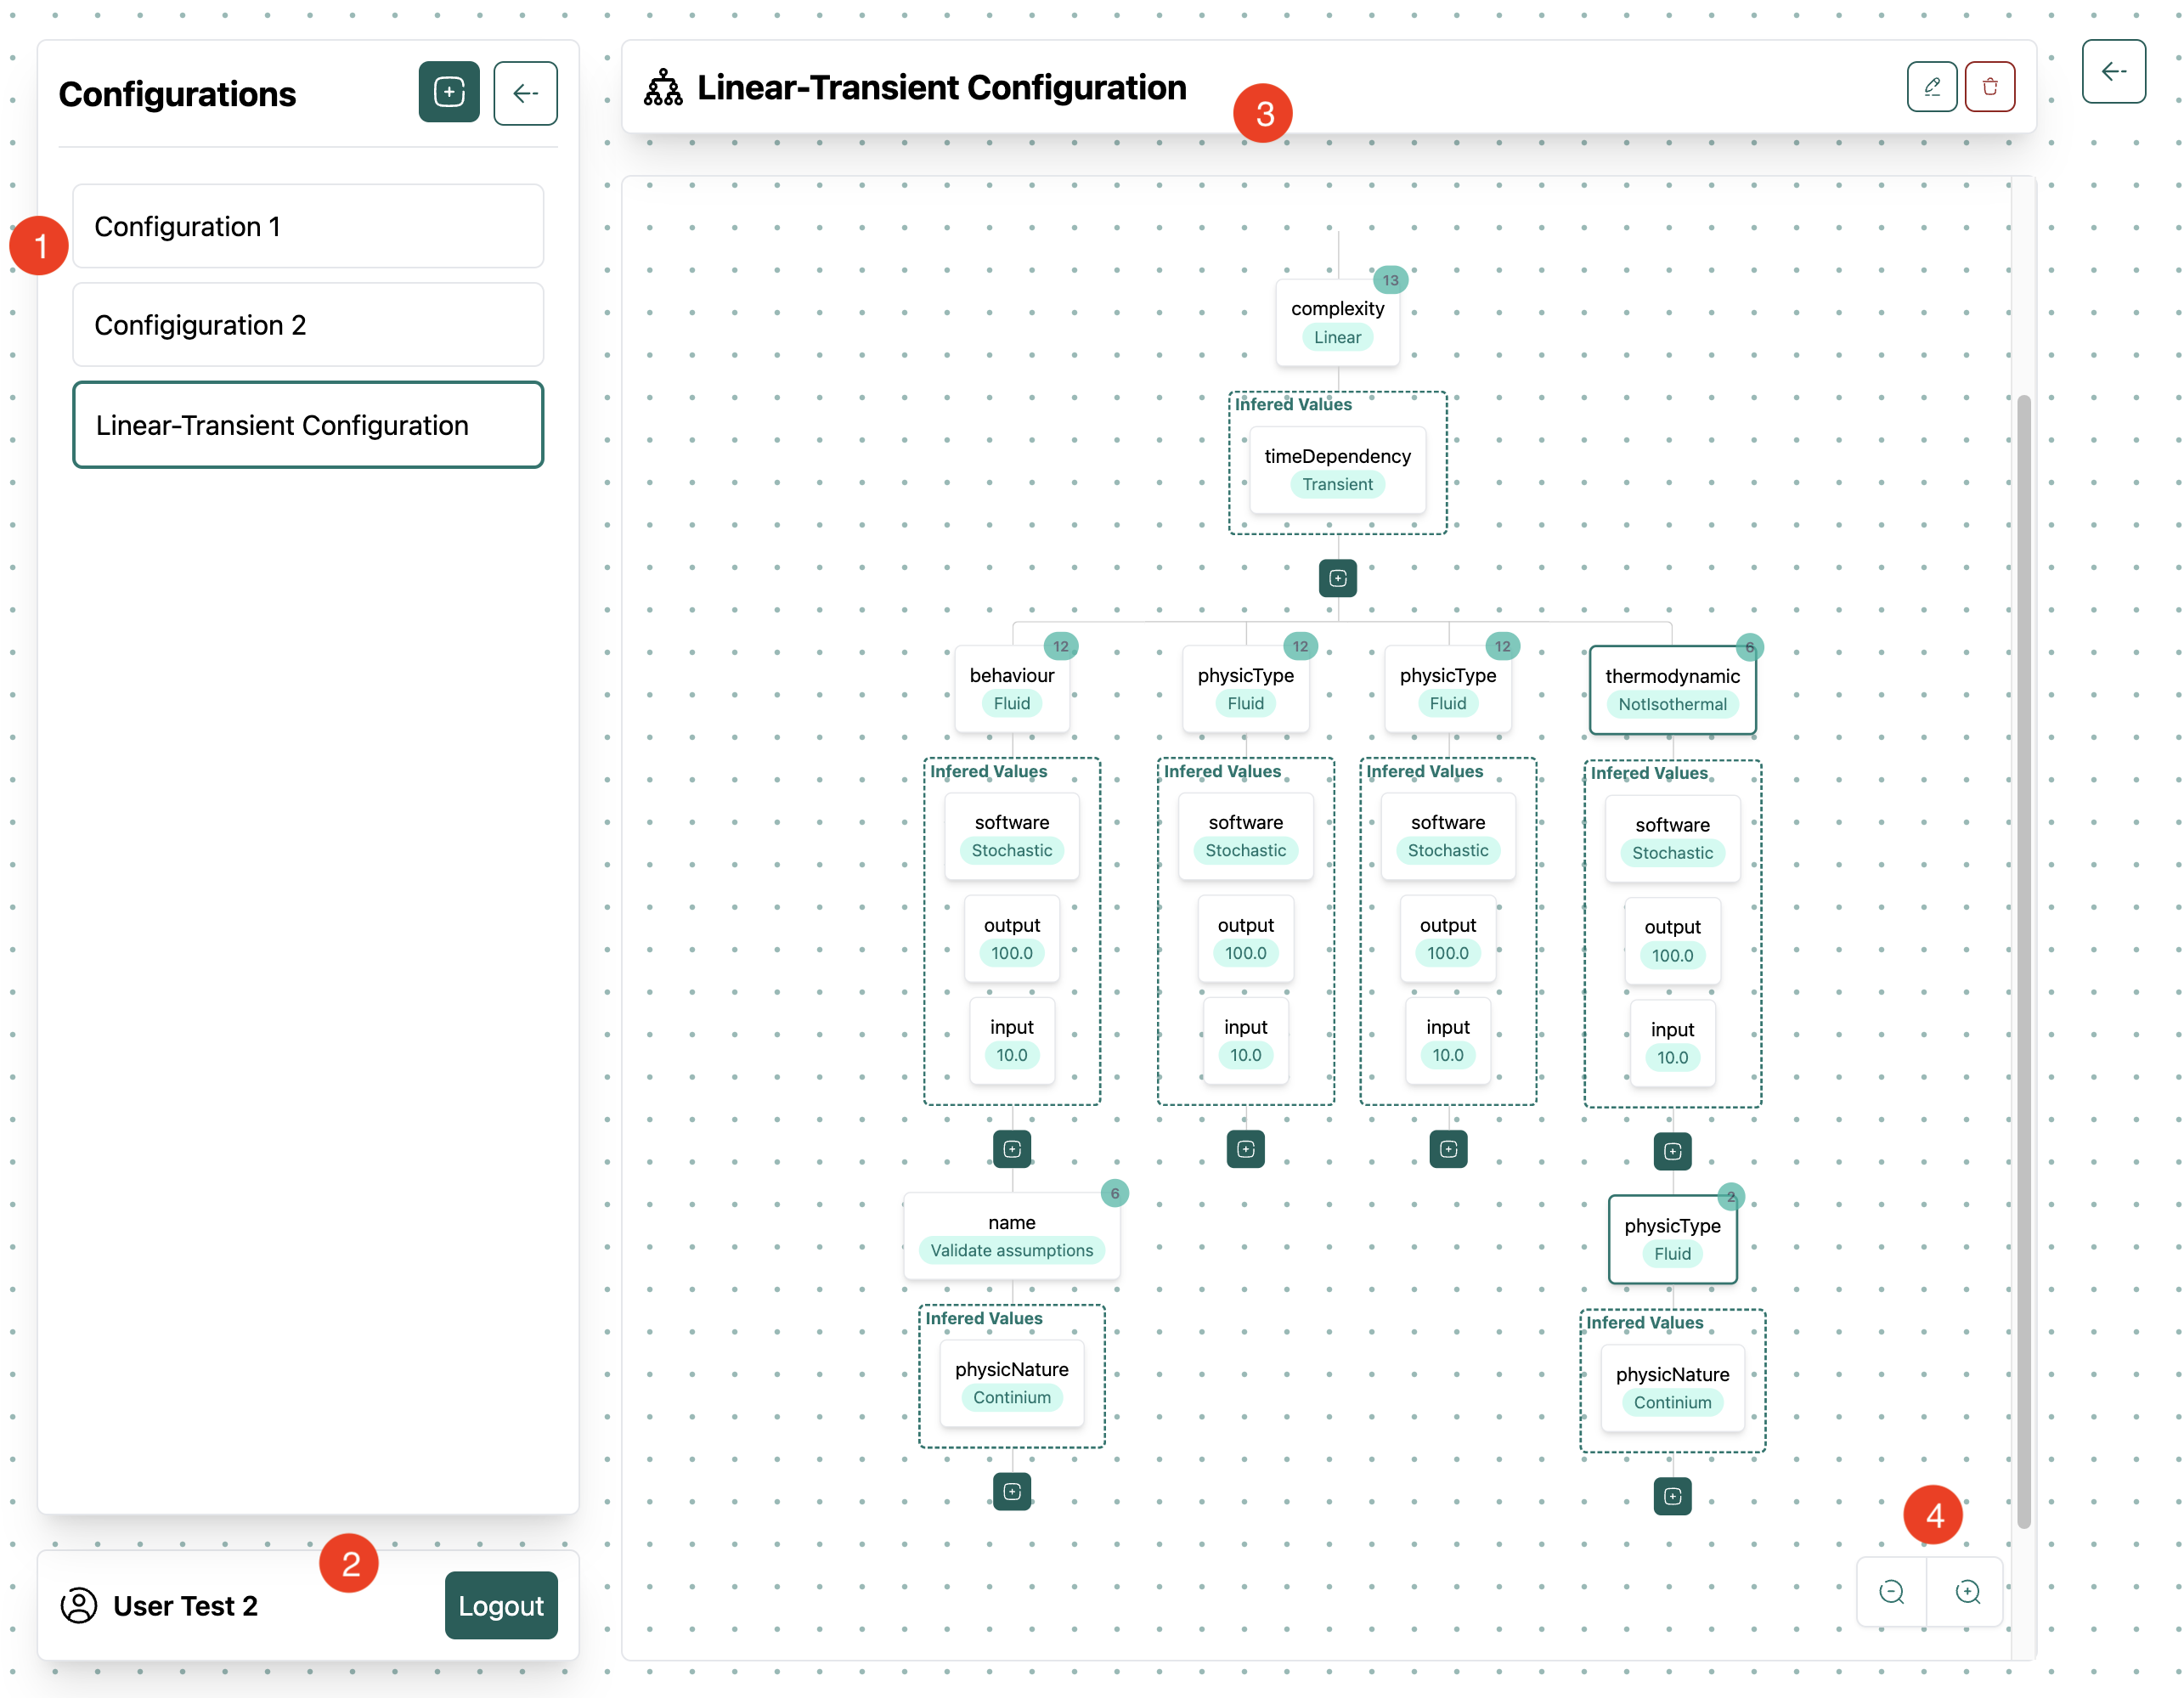
\includegraphics[width=\textwidth]{images/proto-demo.png}}
    \caption{\label{fig:proto-demo}  Main view of the \acrshort{ui} prototype}
    \end{figure}
    
    
    \subsubsection{Answering to question}
    To add an answer to the tree, simply click on the “+” button below a Node. Figure\ref{fig:proto-demo-add-answer} shows the dialogue box that appears once you have clicked on this button. This dialogue box contains:
    
    \begin{itemize}
        \item \textbf{(1)} an entry for selecting the element for which you would like to give a value
        \item \textbf{(2)} an entry for giving the value of this element. As shown in Figure\ref{fig:proto-demo-add-answer-proba} a suggestion of possible values is automatically made. And for each of the suggested values, a probability of use is provided, allowing you to find out how many similar simulations have used this value.
        \item a “mandatory” switch \textbf{(3)} to define whether only graphs with exactly the value selected for the element selected should be taken into account
        \item In \textbf{(4)} we have the question asked for this element. This is generated automatically by the backend.
    \end{itemize}
    

    \begin{figure}[h]
        \centering
        \begin{subfigure}[b]{0.45\textwidth}
            \centering
            \frame{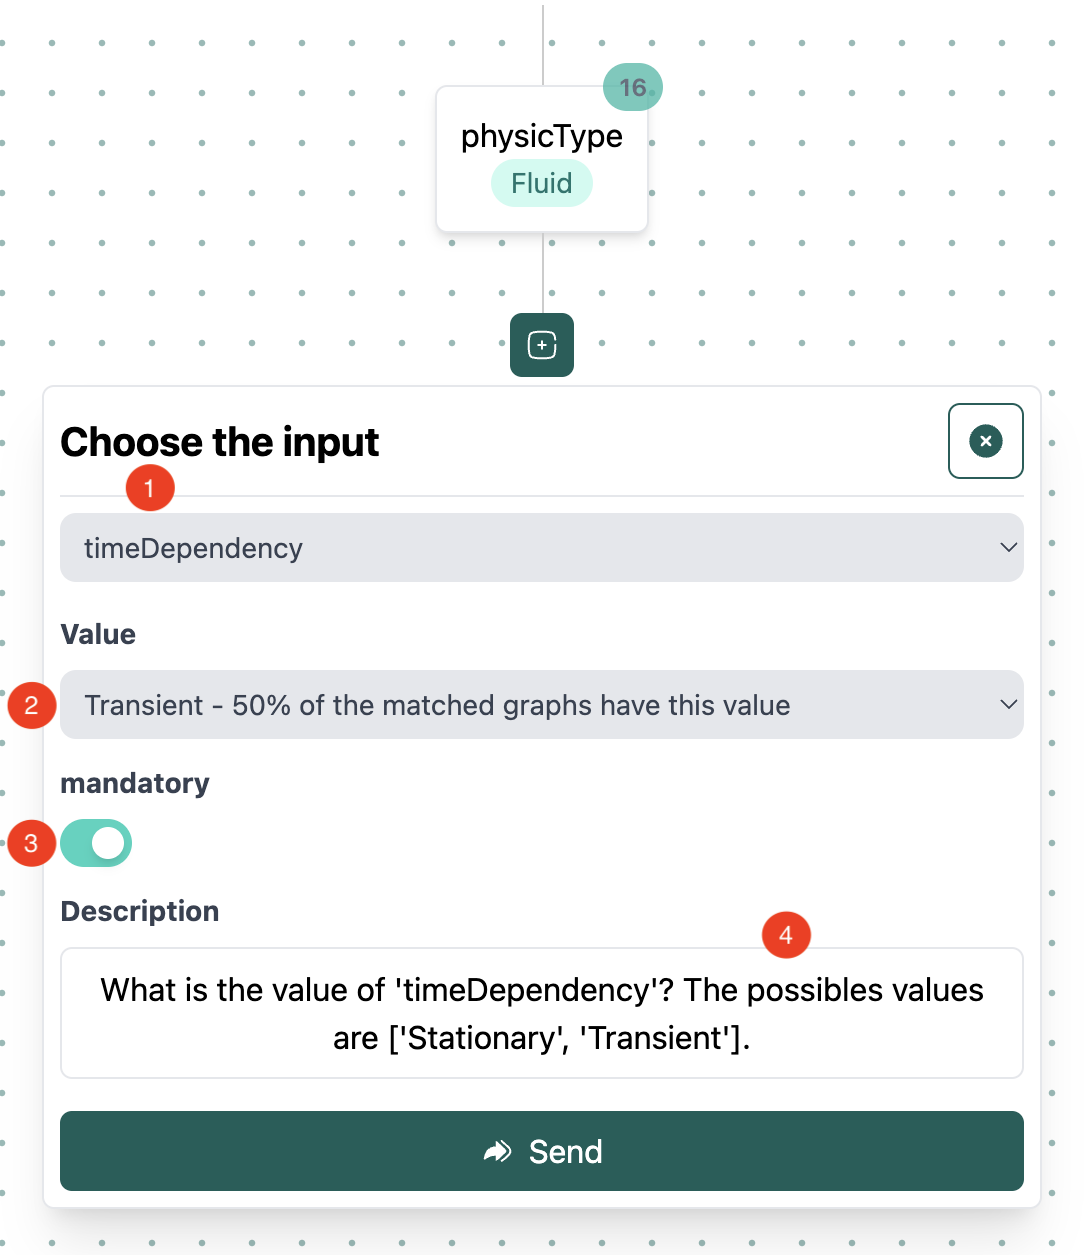
\includegraphics[width=\textwidth]{images/proto-demo-add-answer.png}}
            \caption{\label{fig:proto-demo-add-answer} Dialog to answer to a question}
        \end{subfigure}
        \begin{subfigure}[b]{0.45\textwidth}
            \centering
            \frame{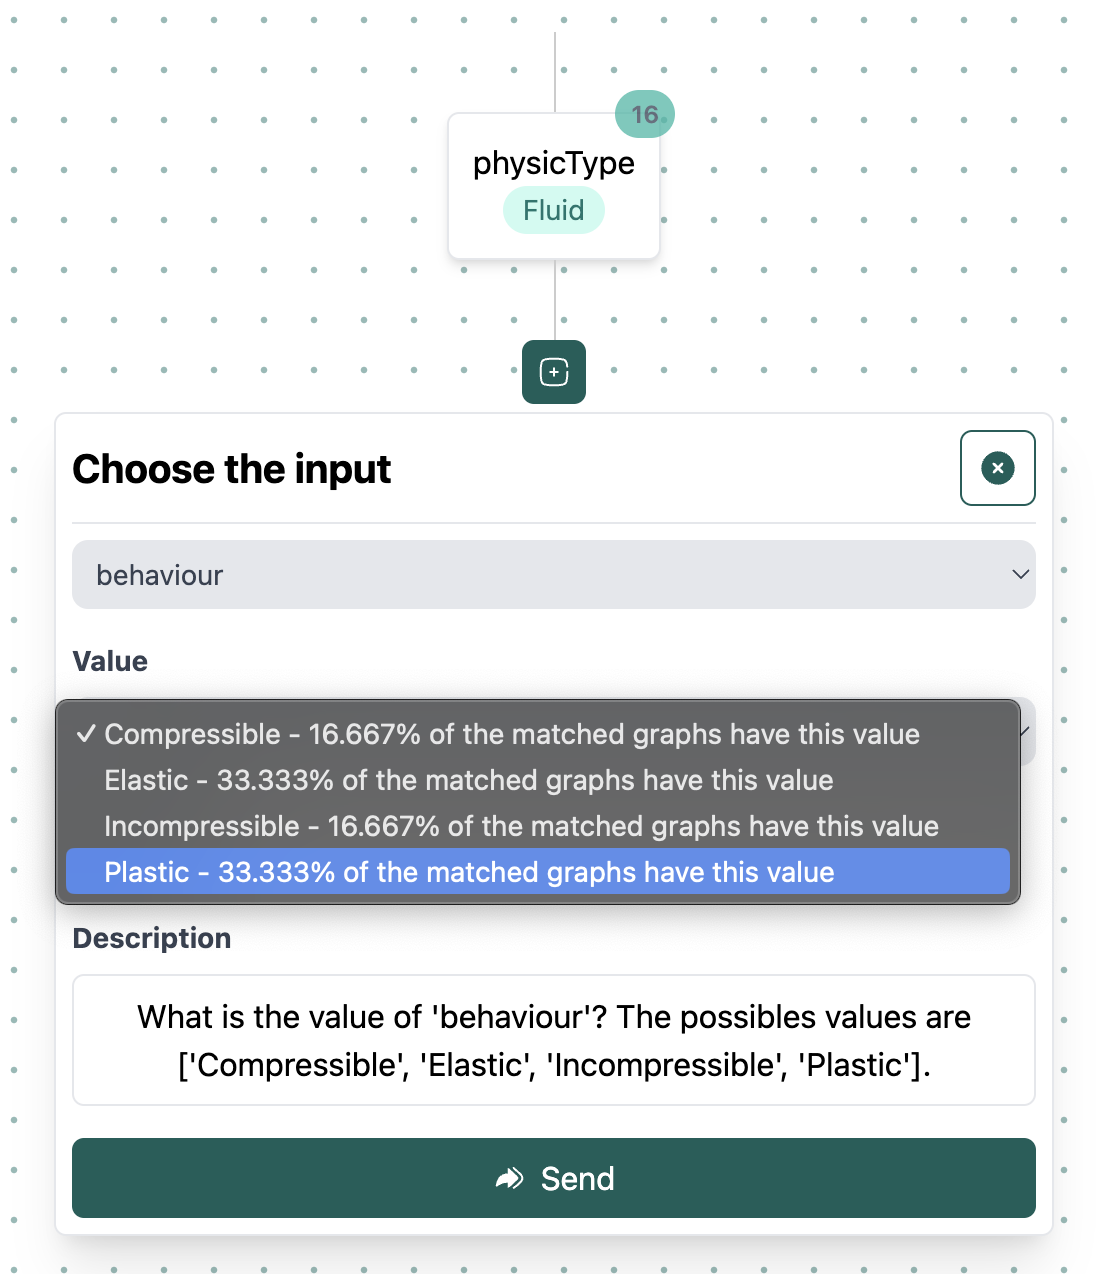
\includegraphics[width=\textwidth]{images/proto-demo-add-answer-proba.png}}
            \caption{\label{fig:proto-demo-add-answer-proba} Probability of usage}
        \end{subfigure}
    \end{figure}
    
    
    \subsubsection{Edit / Delete an answer}
    It is also possible to edit or delete an answer given previously. Figure\ref{fig:proto-demo-edit-delete-answer} shows the elements of our interface which allow this to be done. 
    
    \begin{itemize}
        \item when a Node (response) in the graph is edited, this automatically deletes all the child Nodes it had, since these may no longer be relevant for the new values of the modified Node
        \item when a Node is deleted, its child Nodes are also deleted
    \end{itemize}

    \begin{figure}[h]
    \centering
    \frame{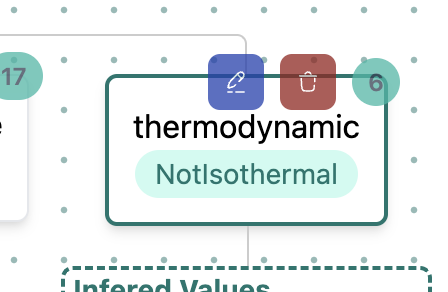
\includegraphics[scale=0.5]{images/proto-demo-edit-delete-answer.png}}
    \caption{\label{fig:proto-demo-edit-delete-answer}  Edit / Delete an answer (a Node)}
    \end{figure}

    
    \subsubsection{Inspecting results}
    After each response, the reasoner recalculates the similar simulations and returns them. You can see the number of simulations found in the top right-hand corner of each Node. For more details, simply click on the Node you wish to inspect. Figure\ref{fig:proto-demo-detail} shows the details of one of these Nodes.
    
    \begin{itemize}
        \item In \textbf{(1)} we have information about the number of simulations found.
        \item The selection list \textbf{(2)} allows you to choose one of the simulations found in order to inspect it.
        \item Once one of the simulations has been chosen, we can see the percentage of similarity \textbf{(3)} of this simulation with the one currently being configured.
        \item The table in \textbf{(4)} shows all the attributes of this simulation and their values.
    \end{itemize}
    
    \begin{figure}[h]
    \centering
    \frame{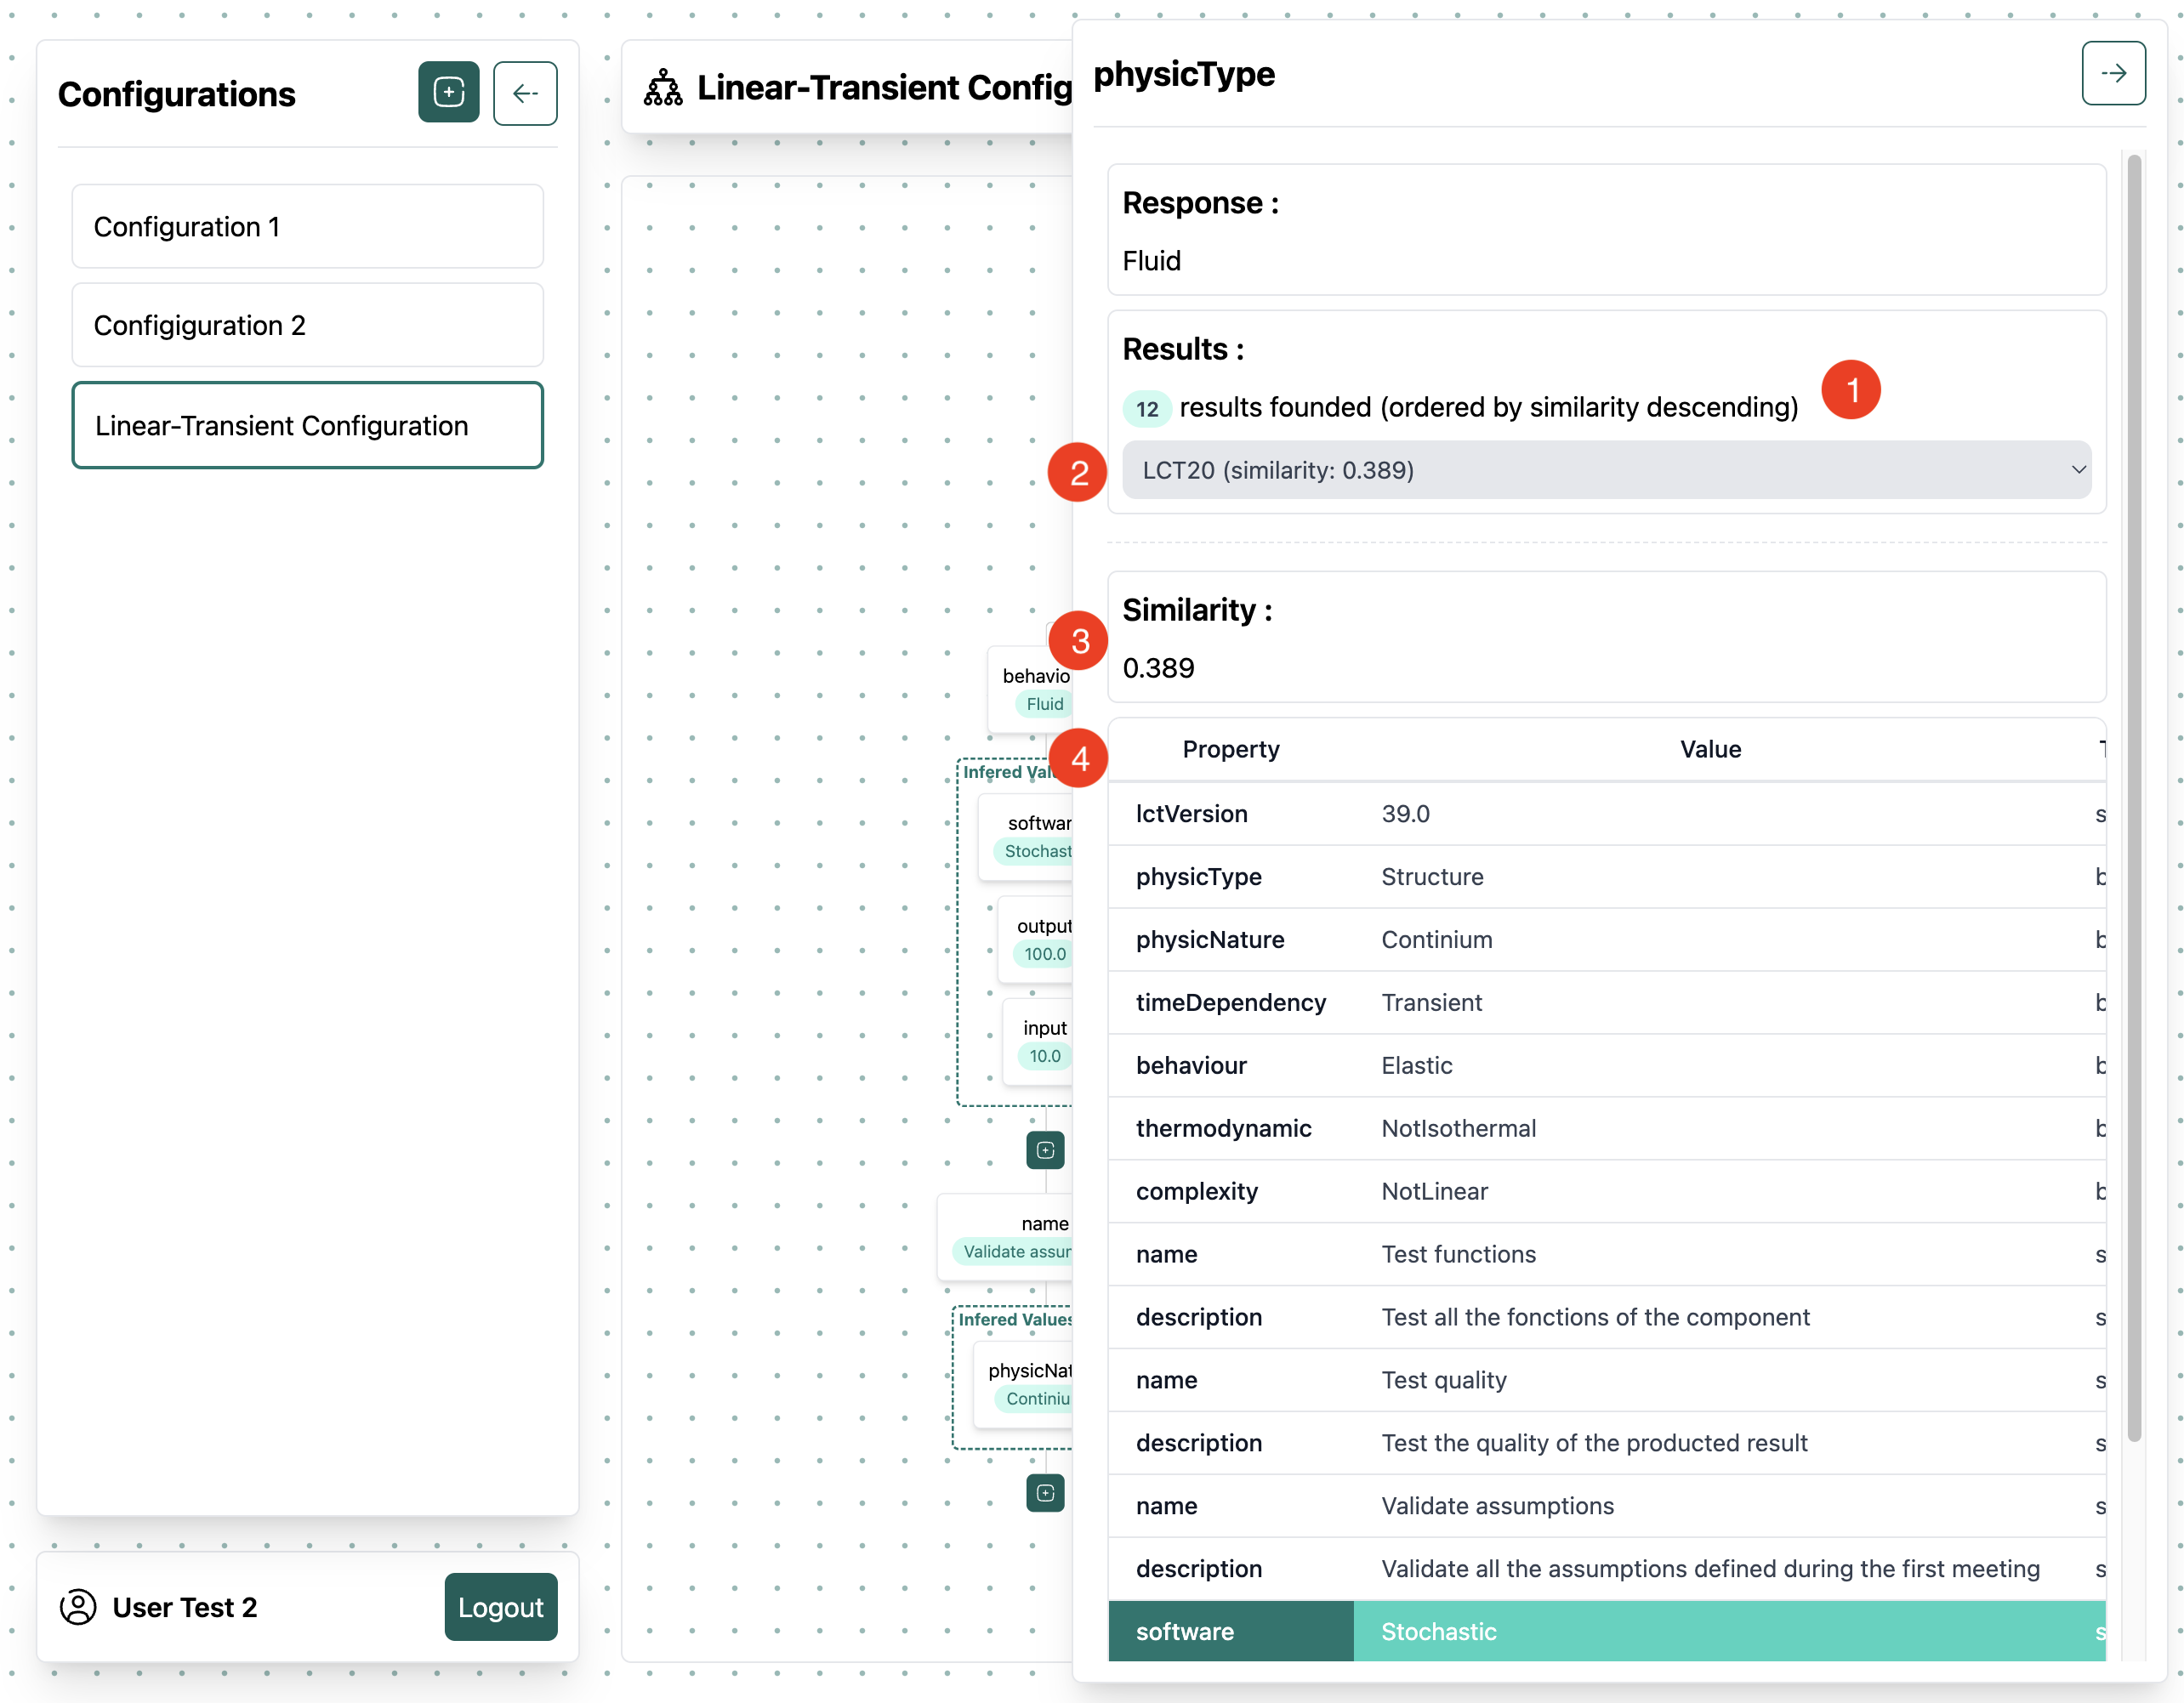
\includegraphics[width=\textwidth]{images/proto-demo-detail.png}}
    \caption{\label{fig:proto-demo-detail}  Inspect the details of a node}
    \end{figure}




    